\documentclass[
    a4paper,
    fontsize=12pt,
    footinclude=true,
    headinclude=true
	]{scrbook}

	\usepackage{scrhack}
	\usepackage{silence}
	\WarningFilter{latex}{You have requested package}
	\usepackage{template/preamble}
	\setlength{\parskip}{0.3em}

\bibliography{biblio.bib}








\usepackage{ifthen}
\usepackage{adjustbox}
\usepackage{graphicx}
\usepackage{comment}
\usepackage{svg}
\usepackage{amsmath,amssymb} % define this before the line numbering.
\usepackage{color, colortbl}
\usepackage[dvipsnames]{xcolor}
\usepackage{nicefrac}
\usepackage{booktabs}
\usepackage{placeins}
\usepackage{pifont}
\usepackage{subcaption}
\usepackage{xspace}
\usepackage{gensymb}
\usepackage{arydshln}
\usepackage{nicefrac}
\usepackage{algorithm}
\usepackage{algpseudocode}
\algrenewcommand\algorithmicindent{1.0em}%
\usepackage{epigraph}
\usepackage{listings}
\usepackage{bibentry}
\usepackage{makecell}
\usepackage{float}


% \usepackage{hyperref}
% \usepackage{xcolor}
% \usepackage[colorlinks=true,linkcolor=black,citecolor=blue,urlcolor=black]{hyperref}



% for an adaptable epigraph
\renewcommand{\epigraphsize}{\small}
\setlength{\epigraphwidth}{0.6\textwidth}
\renewcommand{\textflush}{flushright}
\renewcommand{\sourceflush}{flushright}
% A useful addition
\newcommand{\epitextfont}{\itshape}
\newcommand{\episourcefont}{\scshape}

\makeatletter
\newsavebox{\epi@textbox}
\newsavebox{\epi@sourcebox}
\newlength\epi@finalwidth
\renewcommand{\epigraph}[2]{%
  \vspace{\beforeepigraphskip}
  {\epigraphsize\begin{\epigraphflush}
   \epi@finalwidth=\z@
   \sbox\epi@textbox{%
     \varwidth{\epigraphwidth}
     \begin{\textflush}\epitextfont#1\end{\textflush}
     \endvarwidth
   }%
   \epi@finalwidth=\wd\epi@textbox
   \sbox\epi@sourcebox{%
     \varwidth{\epigraphwidth}
     \begin{\sourceflush}\episourcefont#2\end{\sourceflush}%
     \endvarwidth
   }%
   \ifdim\wd\epi@sourcebox>\epi@finalwidth 
     \epi@finalwidth=\wd\epi@sourcebox
   \fi
   \leavevmode\vbox{
     \hb@xt@\epi@finalwidth{\hfil\box\epi@textbox}
     \vskip1.75ex
     \hrule height \epigraphrule
     \vskip.75ex
     \hb@xt@\epi@finalwidth{\hfil\box\epi@sourcebox}
   }%
   \end{\epigraphflush}
   \vspace{\afterepigraphskip}}}
\makeatother


\newcommand{\titlecaption}[3][]{\caption[#2]{\textbf{#2}\ifthenelse{\equal{#1}{}}{. }{ }#3}}

\newcommand{\todo}[1]{\textcolor{BrickRed}{[TODO #1]}}
\newcommand{\note}[1]{\textcolor{PineGreen}{(#1)}}
\newcommand{\review}[1]{\textcolor{RoyalBlue}{#1}}
\newcommand{\startreview}{\color{RoyalBlue}}
\newcommand{\stopreview}{\color{black}}
\newcommand\Tstrut{\rule{0pt}{2.6ex}}         % = `top' strut
\newcommand\Bstrut{\rule[-0.9ex]{0pt}{0pt}}   % = `bottom' stru
\newcommand{\mypm}{\,$\pm$\,}
\newcommand{\mysmpm}[1]{\scriptsize{\mypm#1}}
\newcommand{\minipar}[1]{\noindent \textbf{#1}}
\def\mypar#1{\vspace{1mm}{\noindent\textbf #1}\hspace{1mm}}
\def \ours {{FlexIT}\xspace}


\renewcommand\theadalign{bc}
\renewcommand\theadfont{\bfseries}
\renewcommand\theadgape{\Gape[4pt]}

\definecolor{lightblueborder}{HTML}{41719C}
\definecolor{lightbluefill}{HTML}{5E9CD3}

\let\oldleftmark=\leftmark


\newboolean{skipIntro}
\newboolean{skipRelated}
\newboolean{skipEpipolarNVS}
\newboolean{skipEpiNeRF}
\newboolean{skipGauss}
\newboolean{skipConclusion}
\newboolean{skipAppendix}

% By setting this to true, you skip the compiling of some chapters
\setboolean{skipIntro}{false}
\setboolean{skipRelated}{false}
\setboolean{skipEpipolarNVS}{false}
\setboolean{skipEpiNeRF}{true}
\setboolean{skipGauss}{true}
\setboolean{skipConclusion}{true}
\setboolean{skipAppendix}{true}

%\mtcsetoffset{minitoc}{-0.80em}

\setlength{\mtcindent}{-0.80em}

\begin{document}

\tracingall

\dominitoc
\selectlanguage{english}


\frontmatter



\begin{titlepage}

  \vspace*{-2.5cm}
  \includegraphics[height=0.1\columnwidth]{images/saclay.png}
  \hspace*{.5cm}
  \includegraphics[height=0.1\columnwidth]{images/meero.jpg}
  \hspace*{.5cm}
  \includegraphics[height=0.1\columnwidth]{images/cea_list.png}
  \vspace*{0.5cm}

  \begin{center}

    {\large \textbf{T\normalsize{HÈSE DE}\large{} D\normalsize{OCTORAT DE}\large{} P\normalsize{aris}\large{}-S\normalsize{aclay}\large{} U\normalsize{NIVERSITÉ}}}\\
    \textbf{Pôle B} : Données, connaissances, apprentissage et interactions \\
    École Doctorale Sciences et Technologies de l'Information et de la Communication (Paris-Saclay)

    \vspace*{1.5cm}

    {\Large \textbf{Novel View Synthesis through 3D considerations}} \\[0.5em]
    {\large \textbf{Synthèse de Nouvelles Vues via des considérations 3D}}

    \vspace*{1.2cm}

    Présentée par\\
    {\large \textbf{Gaétan {Landreau}}}

    \vspace*{2mm}

    Dirigée par\\
    \textbf{Dr. Mohamed {Tamaazousti}}

    \vspace*{5mm}

    Pour obtenir le grade de \ \\
    \textbf{DOCTEUR de Paris-Saclay UNIVERSITÉ} \ \\

    \vspace*{5mm}

  \end{center}

  \definecolor{mygray}{gray}{0.37}
  \newcommand{\affil}[1]{\multicolumn{2}{@{\hskip 18pt}l@{}}{\small \itshape \textcolor{mygray}{#1}}}

  %\vspace*{5mm}
  \flushleft{
    Présentée et soutenue publiquement le - 2024 \\[2mm]
    Devant le jury composé de :\\[2mm]
    \begin{tabularx}{\textwidth}{@{\hskip 18pt}Xr}
      Dr. Paul \textsc{Jacques} & Rapporteur                 \\[-0.5mm]
      \affil{Directeur de recherche, Laboratoire de } \\[0.5mm]
    \end{tabularx}
    \begin{tabularx}{\textwidth}{@{\hskip 18pt}Xr}
      Dr. Paul \textsc{Jacques} & Rapporteur \\[-0.5mm]
      \affil{Directeur de recherche, Laboratoire de }    \\[0.5mm]
    \end{tabularx}
    \begin{tabularx}{\textwidth}{@{\hskip 18pt}Xr}
      Pr. Paul \textsc{Jacques} & Examinatrice        \\[-0.5mm]
      \affil{Professeur des université, } \\[0.5mm]
    \end{tabularx}
    \begin{tabularx}{\textwidth}{@{\hskip 18pt}Xr}
      Pr. Paul \textsc{Jacques} & Examinateur \\[-0.5mm]
      \affil{Maître de Conférences, } \\[0.5mm]
    \end{tabularx}
    \begin{tabularx}{\textwidth}{@{\hskip 18pt}Xr}
      Pr. Paul \textsc{Jacques} & Examinateur          \\[-0.5mm]
      \affil{Maître de Conférences, } \\[0.5mm]
    \end{tabularx}
    \begin{tabularx}{\textwidth}{@{\hskip 18pt}Xr}
      Dr. Mohamed \textsc{Tamaazousti} & Directeur de thèse \\[-0.5mm]
      \affil{Researcher,CEA List}          \\[0.5mm]
    \end{tabularx}
    \begin{tabularx}{\textwidth}{@{\hskip 18pt}Xr}
      Florian \textsc{Köning} & Invité \\[-0.5mm]
      \affil{Research Scientist, CarCutter by Meero} \\[0.5mm]
    \end{tabularx}

  }
  %}

\end{titlepage}
\thispagestyle{empty}

\hfill

\vfill

\noindent\myName: \textit{\myTitle,}
\textcopyright\ 2024


% TOC

% \acused{AE}
% \acused{SHADE}
% \acused{SWWAE}
% \acused{HySWWAE}
\microtypesetup{protrusion=false}
\cleardoublepage
\addcontentsline{toc}{chapter}{\texorpdfstring{\noexpand\spacedlowsmallcaps{\contentsname}}{\contentsname}}
\setcounter{tocdepth}{1}
\setcounter{minitocdepth}{2}
\setcounter{secnumdepth}{3}
\manualmark
\markboth{\spacedlowsmallcaps{\contentsname}}{\spacedlowsmallcaps{\contentsname}}
\tableofcontents
\adjustmtc
\automark[section]{chapter}
\renewcommand{\chaptermark}[1]{\markboth{\spacedlowsmallcaps{#1}}{\spacedlowsmallcaps{#1}}}
\renewcommand{\sectionmark}[1]{\markright{\thesection\enspace\spacedlowsmallcaps{#1}}}
\microtypesetup{protrusion=true}


% list of tables and list of figures

% \cleardoublepage
% \addcontentsline{toc}{chapter}{\texorpdfstring{\noexpand\spacedlowsmallcaps{\listfigurename}}{\listfigurename}}
% \listoffigures
% \adjustmtc

% \cleardoublepage
% \addcontentsline{toc}{chapter}{\texorpdfstring{\noexpand\spacedlowsmallcaps{\listtablename}}{\listtablename}}
% \listoftables
% \adjustmtc

\cleardoublepage
\setcounter{page}{1}

\chapter{Abstract}
Back in computing history, \ac{NVS} is a new and emergent field which roughly appear during the 1990s. Blending computer graphics, 3D reconstruction and computer vision, \ac{NVS} aims to generate images of a scene from unobserved viewpoints. Whereas recent breakthrough of so-called \textit{deep learning} based methods allowed substantial advancements since 2010s, the domain keeps leveraging on its old concepts, from multi-view geometry to 3D reconstruction. Given its numerous potential applications \ac{NVS} is nowadays at the spotlight of attention, from \ac{VR} and \ac{VR}, to 3D rendering, and thus naturally to video games or animation.

We chose to adress in this thesis one of the most constraintful scenario in \ac{NVS}, by only relying on a single image as input. 

First part of this manuscript focuses on the way camera pose information can be encoded and thus provided as an apriori to a \ac{NN} through epipolar considerations. Indeed, such camera pose information, that thus account for the relative displacement that occured between the given source view and the target one we aim to generate, is often sub-optimally encoded. We show through our work that such camera pose can be entirely encoded in an image, thanks to epipolar lines. 

We highlight in a second part how \ac{NeRF} completely changed the way \ac{NVS} was adressed until now. Such architecture now has appealing generative properties, that therefore allow to synthesize novel views without being limited to a unique scene. However, epipolar constraints integration in these networks is still relatively untouched. We proposed an effective yet simple feature based attention mechanism, relying on a second \ac{NeRF}. 

Finally, we relax our initial constraint on the single view to get closer to an industrial application of \ac{NVS}. Given multiple images, \ac{GS} models accurately reconstruct apparence and 3D geometrical structures of any scene. Yet, performing rendering of these scene at unobserved location lead to severe artifacts that must be removed, while stabilizing the new camera trajectory as well as possible. 

\cleardoublepage


\chapter{R\'esum\'e}
\selectlanguage{french}

La synthèse de nouvelles vues est un domaine relativement récent dans l'histoire de l'informatique, qui remonte approximativement aux année 90. Mélant infographie, reconstruction 3D et vision par ordinateur,la synthèse de nouvelles vues cherche à générer des images d'une scène depuis des angles de vue non observés au préalable. Si l'avénement des techniques d'apprentissages dites \textit{profondes} a permis de réelles avancés significatif sur ce sujet depuis 2010, le domaine garde toujours ces anciens fondements, de la géométrie multi-vues à la reconstruction 3D. La synthèse de nouvelles vues est aujourd'hui au coeur de toutes les attentions, tant ses applications potentielles sont nombreuses, de la \ac{RV} et l'\ac{RA}, en pasant par le rendu 3D, et donc naturellement les jeux vidéos ou encore l'animation.

Nous adressons dans cette thèse l'une des configurations les plus contraignantes en synthèse de nouvelles vues, en se cantonnant à n'avoir en entrée qu'une vue unique. 

La première partie de ce manuscrit s'intéresse à la manière dont l'information de pose de caméra peut être encodée et fournie comme apriori d'information à un réseau de neurone via des considérations issues de la géométrie épipolaire. En effet, cette information de pose, traduisant le déplacement relatif entre la vue d'entrée et celle à générer, est souvent encoder de manière sous optimal. Nous montrons à travers nos travaux que cette pose peut être intégralement encodée dans une image, grâce aux droites épipolaires. 

Nous montrons dans un second temps comment l'avénement récent des \ac{NeRF} a complètement redistribué la manière d'adresser la synthèse de nouvelles vues. Ce type d'architecture possède désormais des propriétés génératives intéressante, qui permettent donc synthétiser de nouvelles vues sans se limiter à une scène unique. Cependant, l'intégration de contraintes épipolaires dans ces réseaux est encore assez peu explorée, et proposons donc un mécanisque d'attention simple, basé sur des attributs issu d'un second \ac{NeRF}. 

Enfin, dans une dernière partie, nous élargissons et relaxons notre contrainte initiale pour s'approcher davantage d'une application industrielle. En se donnant davantage de vues, les modèles de types \ac{GS} permettent de reconstruire fidèlement l'apparence et la structure géométrique 3D d'une scène. Pourtant, rendre ces scènes à des positions éloignés des vues originellement observés donne lieu à de multiples artifacts, qu'il convient de supprimer, tout en stabilisant au mieux nouvelle la trajectoire de la caméra. 

\selectlanguage{english}

\cleardoublepage
\chapter{Acknowledgments}


% \selectlanguage{english}




\cleardoublepage
\faketableofcontents
\chapter{Acronyms}\label{chap:acronyms}



\begin{acronym}[XXXXXXX]
    \acro{AI}{Artificial Intelligence}
    \acro{AR}{Augmented Reality}
    \acro{CNN}{Convolutional Neural Network}
    \acro{DNN}{Deep Neural Networks}
    \acro{DL}{Deep Learning}
    \acro{FPS}{Frames Per Second}
    \acro{GAN}{Generative Adversarial Network}
    \acro{GPU}{Graphics Processing Unit}
    \acro{GenAI}{Generative AI}
    \acro{GS}{Gaussian Slatting}
    \acro{LLM}{Large Language Model}
    \acro{NN}{Neural Network}
    \acro{NVS}{Novel View Synthesis}
    \acro{MAE}{Mean Average Error}
    \acro{MPI}{Multi Plane Images}
    \acro{NeRF}{Neural Radiance Fields}
    \acro{SSIM}{Structural Similarity Index Measure}
    \acro{PSNR}{Peak Signal-to-Noise Ratio}
    \acro{VR}{Virtual Reality}
    \acro{RV}{Réalité Virtuelle} 
    \acro{RA}{Réalité Augmentée}
    \acro{SFM}{Structure From Motion}
    \acro{SH}{Spherical Harmonics}
    \acro{SVD}{Singular Value Decomposition}

\end{acronym}



% % \cleardoublepage
% % \input{content/00_notations.tex}
% % \cleardoublepage

\mainmatter

\chapter{Introduction}
\label{chapter:introduction}

%\minitoc
\chapterwithfigures{\nameref*{chapter:introduction}}
%\chapterwithtables{\nameref*{chapter:introduction}}

\ifthenelse{\boolean{skipIntro}}{\endinput}{}

\emph{Perspicere} - \textit{to see through}. Behind the Perspective's etymology is hidden the notion of portraying our three-dimensional physical reality onto a two-dimensional plane. Such concept has been extensively studied for centuries, and found its oldest fundation in the geometry Euclide defined in his \textbf{Elements} (300BC). Florence, with its artists and architects, paved the way during Quattrocento in Italian Renaissance of linear perspective studies, to represent as accurately as possible surrounding world on paintings and drawings. Brunelleschi (1377-1446) is one the very first that studied how lines, shapes, objects change under different viewpoint observation, at changing angles. Defined with lines of sights that should converge on one or several vanishing points, linear perspective aims to simulate world objects appearance as a viewer's eye would see them.

\begin{figure}[h!]
      \begin{center}
      \includegraphics[width=.8\textwidth]{images/introduction/perugino.jpg}
      \end{center}
      \caption{\textit{The Delivery of the Keys}, 1481–1482, Sistine Chapel, Rome by Perugino (1481–1482). This impressive $3.3m \times 5.5m$ fresco that both illustrated linear perspective and Brunelleschi's architectural style.}
      \label{fig:intro_perugino}
\end{figure}

Even through artistic perspective studies were extremely well-tuned from a technical and mechanical standpoint \citep{simon2021jan}, perspective found new expressions in the scientific realm few centuries later, through the advent of photogrammetry. Notion speaks for itself when we once again at its grec ethymology, \textit{photo} - \ie light -, \textit{gramma} - \ie drawing, writing - and \textit{metron} - \ie measure -. Aimé Laussedat, a French astronomer, geodesist, surveyor and cartographer used the \textit{Hôtel des Invalides} in 1849 to observe, measure and thus try to reproduce physical spaces, lines and objects from multiples perspective views. Whereas photogrammetry therefore leverages parallax effect to extract depth and dimensions from our physical world with observed views, it was intensively used during mid last century for military purposes. The advent of aerial photography, enabled by recent advancements in aviation, allowed for the topographic mapping of entire countries during the Interwar period.

\begin{figure}[h!]
      \begin{center}
      \includegraphics[width=.5\textwidth]{images/introduction/laussedat_phtograpmetrie.png}
      \end{center}
      \caption{Surveyed by the method of graphical intersections applied to perspectives recorded with the camera lucida. Survey of the Château de Vincennes by A. Laussedat, 1850}
      \label{fig:intro_laussedat}
\end{figure}

Photogrammetry has finally been heavily studied through the prism of robotics and computer vision during 1980's, and is somehow today, the very earlier fundamental concept behind \ac{NVS}.

\section{PhD Context}

\subsection{Meero}
Meero is a Software-as-a-Service french startup founded in 2014 that primarily aims to provide \ac{AI}-powered visual enhancement tools and algorithms for businesses across several verticals, from real estate agencies to e-commerce and fashion industries, as well as automotive car dealerships. Meero proposes a wide range of \ac{AI}-based solutions, from sky replacement, virtual staging or object eraser algorithms for the real-estate vertical to background removal or virtual try-on for fashion and e-commerce companies. Regarding its automotive branch, brand as \textit{CarCutter}, Meero offers car dealerships and marketplaces the opportunity to have visually coherent and appealing images. One of its latest product refers as the 360\degree spin, that allow to virtually smoothly turn around a car given a limited set of images. Such a 3D-based application is inherantly covered by \ac{NVS} as soon as unseen viewpoint must be rendered. 

However, fundamental research in computer vision and its conterpart application in industries suffers from a massive gap that needs to be closed: most of academic papers in vision research deal with images that roughly size from $128\times128$ to $1024\times1024$, whereas images from any mobile device now has at least a 2K resolution (up to 4 to 6K for the latest DSLR camera). Even through such claim tends to thin out with latest fundation models and exploding \ac{GPU} compute capabilities, such an image resolution discrepancy prevent, during this thesis, to directly build an image-based \ac{AI} product in industy from an academic vision paper. This thesis somehow tried to filled this gap, mostly by investigating generalizable single-image novel view synthesis architecture, that could thus be non-restricted to a single scene. 

\subsection{3D reconstruction}
 \ac{NVS} is inherently intertwined with 3D reconstruction, as synthesis of novel views was, de facto, allowed when the complete 3D representation of the scene was available, using photogrammetry or Structure-From-X techniques (where X could stands for \textit{Texture, Shading, Silhouette} etc). Using a bunch of different procedures, such as view correlation, triangulation or camera pose estimation, static scenes can be reconstructed in 3D through a set of RGB 3D points from unordered images since a couple of decades. Extracting a textured mesh from it 

\subsection{Novel View Synthesis}


\section{Contributions}
Aiming to perform novel viewpoint synthesis from a single-image is an extremely ill posed-problem since too many details, structures or texture are unobserved on the provided source view. Core problem that thus inherantly rises from the later observation is to find ways, such as efficient pose encoding, structural constraints that bring as many as possible prior information to the \ac{NN}. 

Years before 2023 emergence of \ac{GenAI} and incredibly powerful foundation models \citep{awais2023foundational}, dataset images we dealt with in single-image \ac{NVS} were mostly low resolution, size $128\times128$, as in ShapeNet \citep{ShapeNet}. We tried through this thesis to incorporate, as much as we possibly could, epipolar geometrical constraints and concepts. We were convinced by the same guiding principle for the last three years: \textit{the most fundamental 3D geometric considerations such as epipolar geometry must be explicitly integrated into deep neural networks.}

We tackle the \ac{NVS} problem with several approaches during this thesis, that could be summarized as follow.
\begin{itemize}
      \item \autoref{chapter:epipolarnvs}: \nameref{chapter:epipolarnvs}\\
            We start approaching single-image \ac{NVS} through the prism of camera transformation encoding. Such an information is vital for any \ac{NN} that performs \ac{NVS}, and its integration as a apriori information is far from being trivial. While several approaches exist to feed such intrinsic and extrinsic parameters to a network, we present in this chapter a novel method to encode such a camera transformation, by extensively leveraging on epipolar geometry. The work in this chapter has led to the following conference publication:
            \begin{itemize}
                \item \fullcite{landreau2022epipolarnvs}
            \end{itemize}


      \item \autoref{chapter:epinerf}: \nameref{chapter:epinerf}\\
            We then turn from camera pose encoding to inner 3D constraints consideration in \ac{NeRF}. However, we maintain the epipolar geometry concept in our work and build a feature-based attention mechanism thanks to \ac{NeRF}-based additional network, called \textit{NeRFeature}. Such a mecanism is direclty involved at training time, while we \textit{do not} have access to the target view to build epipolar constraints. Our work is currently in submission:
            \begin{itemize}
                  \item \fullcite{landreau2024epinerf}
            \end{itemize}

      \item \autoref{chapter:gausssplat}: \nameref{chapter:gausssplat}\\
            We finally relaxed the main hypothesis we dealt with in these first two apparoches to work with \ac{NVS} in a multiple-images scenario with 3D \ac{GS}. Such work mostly rely on \textit{CarCutter} 
industrial considerations, as the next generation of the current 360\degree spin stabilization. However, if rendering at training locations goes fine, stabilizing camera path to render unobserved viewpoint, and thus create seamless 360\degree car animation. 
\end{itemize}

\cleardoublepage

\acresetall % flush acronyms so they are redefined completly when first used
\chapter{Related Work}
\label{chapter:related}

% \minitoc


\chapterwithfigures{\nameref*{chapter:related}}
\chapterwithtables{\nameref*{chapter:related}}

\ifthenelse{\boolean{skipRelated}}{\endinput}{}
We give in this chapter a first overview of neural networks as well as neural radiance fields before delving into ... 

\section{Neural Network Learning}

A \ac{NN} can be defined trough 
\section{Neural Radiance Fields}

\subsection{3D reprensentation}\label{section:chapter1_3Drepresentation}

\paragraph{Implicit formulation}

\cleardoublepage
\let\leftmark=\oldleftmark


\acresetall
\chapter{EpipolarNVS: leveraging on Epipolar geometry for single-image NVS} 
\label{chapter:epipolarnvs}

\ifthenelse{\boolean{skipEpipolarNVS}}{\endinput}{}

\newcommand{\tableindent}{\,\,\,\,}
\newcommand{\vt}{\mathbf{t}}

\newcommand{\std}{$\pm\,$}
\newcommand{\clf}{\textit{clf}} \newcommand{\gray}[1]{{\color{darkgray}#1}}

\chapterwithfigures{\nameref*{chapter:epipolarnvs}}
\chapterwithtables{\nameref*{chapter:epipolarnvs}}

\ifthenelse{\boolean{skipEpipolarNVS}}{\endinput}{}

\ac{NVS} can be approached from various data sources perspectives, ranging from a single image to a video sequence, with or without provided camera pose information, by leveraging 3D-based prior information, such as point clouds, or not. The most challenging scenario, which is the focus of this chapter, involves generating a novel viewpoint from a unique source image. However, in this complex case, the latest learning-based solutions often struggle to efficiently integrate the camera viewpoint transformation. Indeed, the extrinsic information is often passed as-is through a low-dimensional vector. In some cases, the camera pose is even quantized using a one-hot representation when parametrized as Euler angles. This vanilla encoding choice prevents the learned architecture from inferring novel views at any viewpoint that was not registered. 

We argue that there is a better way to encode this relative camera pose by leveraging 3D-related concepts, such as the epipolar constraint. We thus introduce in this chapter a method that encodes the viewpoint transformation as a 2D feature image. This camera encoding strategy provides the network with meaningful insights regarding how the camera has moved in space between the two views. By encoding the camera pose information as a finite number of colored epipolar lines, we demonstrate through our experiments that our strategy outperforms vanilla encoding. 

\section{Introduction}

The \ac{NVS} problem can be addressed from different perspectives, depending on available data: number of source images, geometrical priors such as depth or normal maps, 3D scene information trough point cloud, textured meshes, accurate or jittered camera poses etc. We considered in this first chapter one of the most extreme cases for the novel-view synthesis issue. Our work constrains the prediction of a novel viewpoint from a scene by solely leveraging a single source image and the corresponding camera viewpoint transformation. 

Eforts in\ac{NVS} are often oriented toward getting the most visually appealing results, mainly through \ac{NeRF}-based methods \citep{mildenhall2020nerf,wang2021neus,barron2021mip,barron2022mip}. However, only a limited number of works pursue another tricky challenge in \ac{NVS}: investigate a more efficient way to condition a single-image \ac{NVS} architecture on camera pose information. From a general perspective, associated methods often restrict the viewpoint transformation to the extrinsic matrix. Intrinsic is thus discarded since most methods for single-image \ac{NVS} ignore physical image formation properties and do not account for rendering, epipolar geometry or homography concepts. This camera pose conditioning task remains too weakly addressed in the current literature, which motivated us to tackle such an issue in an original way.

While one of the most straightforward solutions to do so consists in encoding the relative camera viewpoint transformation as a feature vector, we claim such a method is sub-optimal, supported by one of the latest state-of-the-art works in monocular depth prediction \citep{zhao2021camera}. We thus propose in this work an innovative solution to encode the camera relative transformation as a 2D feature RGB image, by leveraging epipolar constraints. The new and implicitly encoded camera viewpoint transformation has a similar spatial resolution as the source image, somehow filling the dimensional gap between pose matrices and the RGB space. The contribution we propose in this first chapter is thus three-fold: 
\begin{itemize}
	\item A strategy to encode the camera pose transformation into an implicit feature image builds upon epipolar geometry considerations. 
	\item A neural network architecture that account for this camera viewpoint transformation encoding. 
	\item A spectral loss function that focus onto image highest frequencies to better synthesize complex details.
\end{itemize}

\section{Related work}

\noindent\textbf{Novel view synthesis.} Since modalities involved in \ac{NVS} are diverse (\textit{e.g} images, video sequence, 3D point clouds,meshes, depth or disparity maps, camera poses), various approaches have been explored to adress the novel viewpoint generation challenge. One of the latest trends leverages the power of \ac{NeRF} \citep{mildenhall2020nerf} to render highly realistic scenes from unseen viewpoints \citep{wang2021neus,niemeyer2022regnerf,barron2022mip}. However, in their original formulation, these neural radiance-based  architectures overfir to a single scene and lack generalization capabilities. Recent works \citep{yu2021pixelnerf,li2021mine} have increasingly addressed this limitation by adapting NeRF-based architectures to the single-image \ac{NVS} problem. The next chapter \ref{chapter:epinerf} will also focus on how these generalizable \ac{NeRF} networks can be employed with geometric constraints to tackle this issue. While MINE \citep{li2021mine} is a \ac{MPI} based method that requires accurate ground truth disparity maps, PixelNeRF \citep{yu2021pixelnerf} uses one or multiple input views to render novel viewpoints. Another important area of \ac{NVS} research for indoor navigation uses datasets like RealEstate10K \citep{zhou2018stereo} and Matterport3D \citep{zhao2021camera}. These approaches achieve impressive results with complex architectures \citep{wiles2020synsin,rombach2021geometry,rockwell2021pixelsynth}, but they often rely on hard-to-obtain data, such as ground truth depth maps or dense 3D point clouds.. \newline

\noindent\textbf{Camera pose encoding.} Camera pose can be represented by three degrees of rotations around each world axis and three more for translation, which together define the extrinsic matrix.  Itrinsic parameters, such as focal length or sensor size could also be considered, leading to few more degrees to embed. One straightforward solution encodes viewpoint transformations by computing camera poses difference \citep{sun2018multiview}. Another approach embeds this low-dimentional camera pose information into a higher-dimentional space, as seen in \citep{kim2020novel,rombach2021geometry}. These last two methods can be further simplified using one-hot vectors for camera pose encoding. Finally, the closest work to ours regarding camera pose encoding is \citep{zhao2021camera}. It encodes the camera location (parametrized through a roll and pitch angles as well as a fixed height above a ground plane) as a 2D feature image for predicting depth maps. \newline

\noindent\textbf{Camera pose conditioning.} Extrinsic camera pose is often the only 3D prior information used to condition a neural network for generating novel viewpoints. Based on the camera pose difference $P_{diff}=P_{target}-P_{source}\in \mathbb{R}^{v}$, the authors in \citep{sun2018multiview} tiled this vector across all the pixels of the source RGB image, feeding their \ac{CNN}-based architecture with inputs sized $\mathbb{R}^{H\times W\times (3+v)}$. In contrast, \citep{kim2020novel} used a different strategy by concatenating the camera pose feature vector with the one obtained from their \ac{CNN} encoder before passing it to the decoder. 
Lastly, \citep{wiles2020synsin} designed a single-image \ac{NVS} method that extensively relies on 3D point clouds. The camera viewpoint transformation is applied within the network architecture to update the predicted point cloud before rendering. \newline

\noindent\textbf{Single-image novel view synthesis.} This framework is the most challenging one because minimal information is available during training and inference: a source image and the corresponding camera pose transformation needed to generate the target image. To the best of our knowledge, only a few recent works \citep{sun2018multiview,kim2020novel,yu2021pixelnerf} address this highly constrained setting. While \citep{sun2018multiview, kim2020novel} handle discretized camera transformation (from ShapeNet \citep{chang2015shapenet}, through a unique azimuthal angle since elevation is fixed) and continuous ones (in Synthia \citep{ros2016synthia} and KITTI \citep{geiger2012we} datasets), the pose-feature vector must be adjusted in size accordingly. This adaptability is one of the main benefits of the method we designed. Both discrete and continuous camera transformations are encoded as a featured image with the same resolution as the source image, effectively capturing the real-world transformation between the source and the target views. This property allows us to infer viewpoints, at least for discrete poses, that were not represented within the training set. \newline

\section{Method}
\subsection{Camera viewpoint transformation encoding}
\subsubsection{Epipolar geometry overview }

The general framing of our work can be considered as one of the most challenging, as generating an  image from a different camera viewpoint is only made prior to a single source image and a relative camera transformation. 

We denote the RGB source image as $I_{s} \in \mathbb{R}^{H\times W\times 3}$ and the target view, which we aim to predict, as $I_{t}$.

The pinhole camera model we consider is represented by the intrinsic matrix $K \in \mathbb{R}^{3\times3}$. The rigid motion that accounts for the relative transformation between the source and the target view consists of a rotation $R \in SO(3)$ and translation $T\in \mathbb{R}^{3\times1}$, expressed through the extrinsic parameters of each camera:

\begin{equation}
     \begin{cases}
     R = R_{t} R_{s}^{T} \\
     T = t_{t} - R t_{s}
     \end{cases}
\end{equation}

with $(R_{s},t_{s})$ and $(R_{t},t_{t})$ respectively the source and target camera extrinsics. Epipolar geometry \citep{hartley2003multiple} addresses the projective geometry that connects two camera viewpoints and has various applications such as \ac{SFM} \citep{tamaazousti2011nonlinear}. Epipolar geometry aims to describe the relationship that stands between 3D world location and 2D pixel coordinates, given a stereo pair of cameras and their corresponding poses. The fundamental matrix F is a $3\times3$ matrix that entirely describes such 3D/2D mapping: 
\begin{equation}
    \mathbf{F} = K^{-T} [T]_{X} R  K^{-1}
\end{equation}

with $[.]_{X}$ the skew-symmetric matrix representation of any one-dimensional vector. Given a pixel location\footnote{Homogeneous coordinates are implicitly used here but omitted for clarity reason} $p_{s}\in I_{s}$, such fundamental matrix $\mathbf{F} \in \mathbb{R}^{3\times3}$ allows to define: 
\begin{equation}
    \mathcal{P}_{p_{s}} = \{p_{t}\in I_{t} | p_{t}^{T}\mathbf{F}p_{s} = 0 \}
\end{equation}

as the finite set of pixels from $I_{t}$ that live on the epipolar line defined by $l=\mathbf{F}p_{s}$. From a geometrical viewpoint, such line corresponds to the rendering (on $I_{t}$ camera plane) of the 3D ray that passed through both the camera center of $I_{s}$ and $p_{s}$. 

The fundamental matrix $\mathbf{F}$ establishes a pixel-to-line correspondence through a linear equation involving both the source and the target camera locations. When using epipolar geometry to encode the viewpoint transformation, a sampling strategy must be defined to determine which pixel locations from the source image $I_{s}$ will be used to compute these epipolar lines. Rather than randomly sampling location from the $H\times W$ possibilities, pixels are sampled based on a regular grid $\textbf{G}_{r}$ that spans the entire image, with the parameter \textit{r} controlling the grid’s coarseness: 

\begin{equation}
    \mathbf{G}_{r} = \left\{(p_{x},p_{y}) \in \{1,..,H\}\times \{1,..,W\} \Big\rvert \begin{array}{l}
                    p_x \equiv 0 \pmod{H/r}\\
             p_y \equiv 0 \pmod{W/r}
              \end{array}\right\}
\end{equation}

\subsubsection{Encode the camera viewpoint transformation}

Our module encodes the relative camera motion between the source and target views by leveraging epipolar geometry. Its output is fed into one of the branches of our \ac{NVS} neural network as a feature image that implicitly represents the transformation that has occurred. We denote it as $E_{s\xrightarrow{}t}$.
An overview of the different stages involved in computing $E_{s\xrightarrow{}t}$ is presented in the pseudo-code below in Algorithm \ref{alg:pseudoCode}. \newline

As shown in Algorithm \ref{alg:pseudoCode}, each epipolar line reported on $E_{s\xrightarrow{}t}$ has a distinct color with the sampled pixel from $I_s$. This implementation choice provides additional RGB prior information to the network regarding the color that should be generated, even though lightning issues are not considered. One might notice that the last epipolar lines plotted on $E_{s\xrightarrow{}t}$ may overwrite some previous lines, particularly at specific pixel locations (such as epipoles).Based on our experimental observations, we assert that the order of pixel sampling order (and thus epipolar line overwriting) does not significantly impact the training and inference performance of the model. 

The encoding method depicted here can encode any form of camera viewpoint transformation without requiring structural adaptation. Indeed, most concurrent works need to modify their encoding strategies for viewpoint transformations, as continuous poses are processed differently than discrete ones, where a one-hot encoding strategy might be employed. 

\begin{algorithm}[h!]
    \caption{Epipolar Encoding module \label{alg:pseudoCode}}
    \SetKwInOut{Input}{input}
    \SetKwInOut{Output}{output}
    \SetKwInOut{Parameter}{parameter}
    \SetKwProg{Fn}{Function}{:}{}
    
    \Input{Source image $I_{s}$, Feature map $F$, Set of grid points $\mathbf{G}_{r}$}
    \Output{Epipolar encoded image $E_{s \rightarrow t}$}
    \medskip
    \KwResult{Epipolar encoded image $E_{s \rightarrow t}$}
    
    \Fn{EpipolarEncoding($I_{s}, F, \mathbf{G}_{r}$)}{
        $E_{s \rightarrow t} \gets \textit{zeros}(H, W, 3)$\;
        \For{$p_{G}$ \textbf{in} $\mathbf{G}_{r}$}{
            $colRGB \gets I_{s}[p_{G}]$\;
            \tcp{Build up the set of epipolar lines $\mathcal{P}_{p_{G}}$ for the grid point $p_{G}$}
            \For{$p$ \textbf{in} $\mathcal{P}_{p_{G}}$}{
                $E_{s \rightarrow t}[p] \gets colRGB$\;
            }
        }
        \Return $E_{s \rightarrow t}$\;
    }
\end{algorithm}

Only non-null pixel values are sampled from $\textbf{G}_{r}$ in our encoding strategy for ShapeNet \citep{chang2015shapenet}, as pixels located in the background do not provide valuable information regarding the corresponding colored epipolar lines. Figure \ref{fig:examplePoseEncoded} illustrates the kind of results one might expect with our viewpoint camera transformation encoding strategy on ShapeNet \citep{chang2015shapenet}. 
\begin{figure}[h!]

\begin{center}
\includegraphics[width=.26\textwidth]{images/epipolarnvs/Is_ECML.png}\hspace{.5cm}%\hfill
\includegraphics[width=.26\textwidth]{images/epipolarnvs/It_ECML.png}\hspace{.5cm}%\hfill
\includegraphics[width=.26\textwidth]{images/epipolarnvs/Est_ECML.jpg}
\end{center}
\caption{\textbf{Pair of source/target image with our encoded transformation.} From left to right: Source image $I_s$, Target image $I_t$ and the corresponding $E_{s\xrightarrow{}t}$. From the ShapeNet \citep{chang2015shapenet} \textit{chair} class. Pixel locations sampled from $\textbf{G}_{25}$ are highlighted with red circles.}
\label{fig:examplePoseEncoded}
\end{figure}


\subsubsection{Extended strategy for real-world camera transformation encoding}

Performing \ac{NVS} on Synthia \citep{ros2016synthia} and KITTI \citep{geiger2012we} datasets is redundant and challenging from the perspective of relative camera transformation within our encoding framework. The images from this dataset were recorded from a car driving through city streets. Consequently, the relative transformations between source views and target views are often pure translations. Such viewpoint changes between the source and target views are inadequately handled by epipolar theory, as depth cues are lost. Therefore, we extended our initial encoding strategy for these datasets by introducing a fourth channel that specifically accounts for depth information.

Let's denote:
\begin{equation}
    \Delta_{t}= |t_{t}| - |t_{s}| = \left[\Delta t_{X},\Delta t_{Y},\Delta t_{Z} \right]^{T} \in \mathbb{R}^3
    \label{eq:delta_t}
\end{equation}
the difference between the two absolute translations $t_s$ and $t_t$. Absolute values are taken in Equation \eqref{eq:delta_t} since 2D planes coordinates are not standardised across scenes in KITTI \citep{geiger2012we} and Synthia \citep{ros2016synthia}. The meaningful scalar value of interest is referred as $\delta_{t}$ and is computed through:
 
 \begin{equation}
 \label{eq:2}
     \delta_{t} = sign(t_{M}) \times| t_{M} |
 \end{equation}
 with 
 \begin{equation}
    t_{M} = \Delta_{t}\left[p_{M}\right] \quad ; \quad p_{M}= \argmax|\Delta_{t}|
\end{equation}

The expression of $\delta_{t}$ satisfies two important constraints in our case: 

\begin{itemize}
    \item It accounts for the primary direction of car motion and provides insight into the distance the car moved between the source and target view.
    \item The sign of $\delta_{t}$ indicates whether the sampled source/target frames correspond to a forward or backward motion.  
\end{itemize}
These properties enable the network to better understand the direction of the motion it should consider. The value of  $\delta_{t}$ is ultimately stored in a fourth channel of $E_{s\xrightarrow{}t}$ only at locations where the epipolar lines have non-zero values in the first three RGB channels. 

\begin{figure}[htpb!]
    \centering
    \begin{subfigure}[b]{0.48\linewidth}
      \includegraphics[width=\linewidth]{images/epipolarnvs/XYplaneMotionKITTI.png}
      \caption{Sequence \textbf{00}}
    \end{subfigure}
    \quad % Space between the figures
    \begin{subfigure}[b]{0.48\linewidth}
      \includegraphics[width=\linewidth]{images/epipolarnvs/XYplaneMotionKITTI01.png}
      \caption{Sequence \textbf{01}}
    \end{subfigure}
    \caption{\textbf{Car displacement in (XY) plane.} We illustrate below the overall trajectory in the (XZ) plane of the car that drove across German's street to acquire the 00 and 01 sequences of the KITTI ~\citep{geiger2012we} dataset.}
    \label{fig:test}
  \end{figure}

  
As shown in Figure \ref{fig:test}, most car trajectories follow a straight path, with only a few turns in sequence \textbf{00}. Similarly, sequence \textbf{01} is nearly a complete end-to-end pure translation.

\subsection{Neural network architecture and training losses}

The overall network architecture is presented in Figure \ref{fig:architecture}. This architecture is inspired by the one introduced by \citep{kim2020novel}, particularly regarding the image-to-image U-Net based encoder/decoder structure with the hard-flow attention strategy. However, the way transformation viewpoint information is provided to our network architecture differs significantly from the base model. While \citep{kim2020novel} concatenates feature vectors within the bottleneck stage of the \ac{CNN}, we argue that this choice is suboptimal for discrete camera pose information contained in ShapeNet \citep{chang2015shapenet}. Instead, we encode this camera pose transformation through $E_{s\xrightarrow{}t}$ as an image that feeds a second \ac{CNN}-based encoder. This encoder produces a feature vector that is concatenated to the one obtained from the RGB U-Net based encoder before being processed by the decoder. 

\begin{figure}[h!]
  \begin{center}
  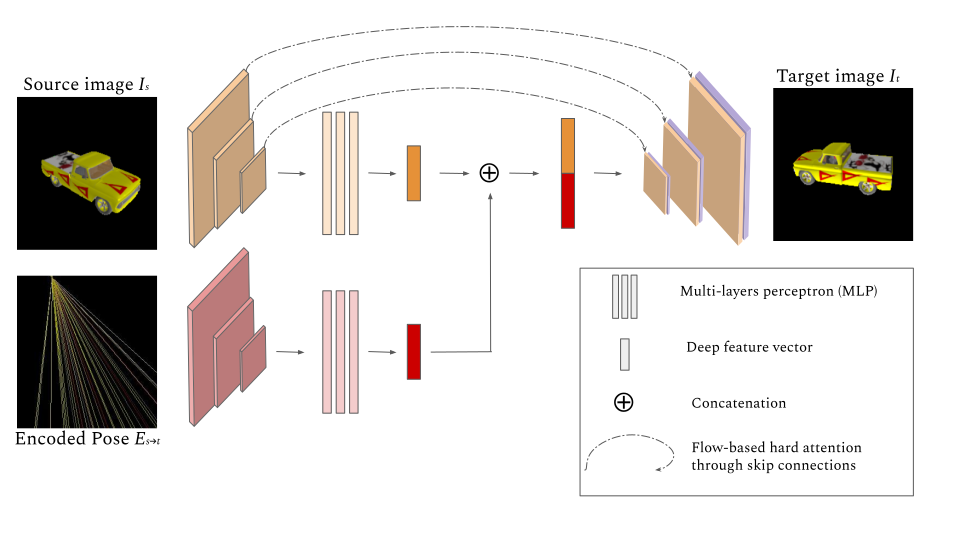
\includegraphics[width=\textwidth]{images/epipolarnvs/NetworkArchitecture.png}
  \end{center}
  \caption{\textbf{General overview of our architecture.} EpipolarNVS takes as inputs both $I_s$ and $E_{s\xrightarrow{}t}$ through two distinct encoders that produce feature vectors that are concatenated before being fed to the decoder. The neural network structure also leverages on the hard flow attention connections introduced in \citep{kim2020novel}.}
  \label{fig:architecture}
\end{figure}

Final loss function is a weighted sum  of a \ac{MAE}, referred as $\mathcal{L}_{1}$, and a second term, called $\mathcal{L}_{spectral}$, directly inspired by prior super-resolution work \citep{fritsche2019frequency}. This latter term extensively focuses on the preserving high frequencies components in the synthesized novel viewpoint. Considering a 2D Gaussian filter $w_{gauss}$, an image $I$ can be decomposed into a low and a high-frequency components, denoted as $I^{LF}$ and $I^{HF}$, respectively. 

\begin{equation}
\begin{cases}
     I^{LF}  = I\circledast w_{gauss} \\
     I^{HF} = I - I^{LF} = (\delta - w_{gauss})\circledast I
\end{cases}
\end{equation}
where $\circledast$ represents a 2D convolution operation. 

The final loss function used during training is thus given by: 
\begin{equation}
    \mathcal{L} = \mathcal{L}_{1} + \lambda \mathcal{L}_{spectral} = |\hat{I}_{t} - I_{t}| + \lambda \left( \hat{I}_{t}^{HF} - I_{t}^{HF} \right)^{2}
    \label{eq:1}
\end{equation}
 \newline

The Gaussian filter $w_{gauss}$ we used is straightforwardly defined by a mean $\mu = \frac{k_{s}-1}{2}$ and a variance $\sigma = (\frac{k_{s}}{k_{s}+1})^{2}$, with $k_{s}$=5.

This spectral term extensively focuses on the highest frequencies of the target and generated images, encouraging the network during training to recover as many fine and complex structures as possible.

\section{Experiments}
All qualitative and quantitative results we obtained through our camera pose encoding strategy are presented in this section. \newline

\noindent\textbf{Datasets.} We trained and tests our method on the \textit{chair} and \textit{car} classes from ShapeNet \citep{chang2015shapenet} as well as on real scene images from KITTI \citep{geiger2012we} and Synthia \citep{ros2016synthia}.
Results we reported for \citep{kim2020novel} slightly differ from the ones originally published by authors since we get consideration for a more challenging rendering scenario. We jittered camera pose in ShapeNet \citep{chang2015shapenet} and image borders from Synthia \citep{ros2016synthia} and KITTI \citep{geiger2012we} were not removed by center-cropping operation. Such changes are motivated and fully exposed in Appendix \ref{annex:epipolarnvs-dataset}.  \newline

\noindent\textbf{Training - Testing.} We trained our model on 100,000 iterations, using the same training procedure as \citep{kim2020novel}. Inference scores were averaged over 100 runs with batch size of 16. \newline

\noindent\textbf{Metrics.} We used the \ac{MAE},  \ac{SSIM} \citep{wang2004image} and \ac{PSNR} metrics to score our single-image \ac{NVS} architecture. 

\subsection{Qualitative Results}

Figure \ref{fig:res_all} presents instances from all the datasets we consider. While our model successfully infers and reasons about object size relative to the target view for the \textit{Car} and \textit{Chair} classes, the novel views produced by \citep{kim2020novel} fails to do so, generating results that roughly match the source object size. Our results on these two classes are also sharper and more realistic, both in term of colour and geometry. For instance, the car's wheels and the chair's intricate back are better synthesized using our method. 

Since \citep{kim2020novel} integrates the camera pose as discretized bins, the viewpoint transformation loses its physical 3D consistency. On the other hand, our method encodes the continuous pose transformation in a way that fully captures the underlying 3D structure.\newline


\begin{figure*}[h!]
    \begin{center}
    \includegraphics[width=\textwidth]{images/epipolarnvs/resultsFinal_BMVC.jpg}
    \end{center}
     \caption{\textbf{Novel view synthesis on the four considered datasets.} Encoded transformation $E_{s\xrightarrow{}t}$ have been obtained with $\textbf{G}_{15}$. From left to right: the source image  $I_s$, $E_{s\xrightarrow{}t}$, \citep{kim2020novel} prediction, our prediction, the target image $I_t$. On overall, our method predicts more consistent results since complete pose transformation has been fed to the network contrary to concurrent work \citep{kim2020novel}. }
     \label{fig:res_all}
\end{figure*}

The results of our method on real-world datasets are shown in the third (Synthia \citep{ros2016synthia}) and fourth (KITTI \citep{geiger2012we}) rows of Figure \ref{fig:res_all}. Notably, in the Synthia \citep{ros2016synthia} dataset, one can observe the car’s motion between the source and target views. While our results remain somewhat blurry, our network successfully hallucinated the forward motion of the bus. Our main concurrent work however replicates the source image and fails to capture the relative displacement in this example. A similar scenario is observed in the KITTI \citep{geiger2012we} dataset. While the sign "30" on the ground disappears between the two views, our method captures this drastic change,  whereas \citep{kim2020novel} stuggles as it did previously. We emphasise the role our camera encoding strategy plays here, especially regarding the shape of various objects where the perspective changes significantly between $I_s$ and $I_t$ (such as the roof of the house in the top-left corner). \newline


While results presented in Figure \ref{fig:res_all} for real world datasets highlight the overall motion that occurred, we focus in Figure \ref{fig:res_all2} on the extent to which high-frequency details are recovered by our model. Although the global motion is reasonably well handled by \citep{kim2020novel}, our method better retrieves tiny details, such as the paintings on the ground. The Spectral loss we used during training helped the network handle these high-frequency details. 

\begin{figure*}[h!]
    \begin{center}
    \includegraphics[width=\textwidth]{images/epipolarnvs/rebbutal_KITTI_3.jpg}
    \end{center}
     \caption{\textbf{Addional inference results on KITTI dataset.} From left to right: the source image  $I_s$, \citep{kim2020novel} prediction, our prediction, the target image $I_t$. Painting on the ground are better reconstructed in our method compared to \citep{kim2020novel}.}
     \label{fig:res_all2}
\end{figure*}

  
\subsection{Quantitative Results}

We present performance results across the four datasets we considered. Tables \ref{tab:1} and \ref{tab:2} respectively summarize the scores for the synthetic ShapeNet \citep{chang2015shapenet} dataset and the real-scene ones (Synthia \citep{ros2016synthia} and KITTI \citep{geiger2012we}). While our method outperforms concurrent approaches on the \ac{MAE} metric, we also achieve highly competitive results on SSIM, with only \citep{sun2018multiview} achieving better scores. \newline

We emphasise on an important aspect regarding the reported scores. Only our method and the one from \citep{kim2020novel} has been retrained with the extended and challenging datasets that we introduced earlier. Results from remaining works \citep{tatarchenko2015single,zhou2016view,park2017transformation,sun2018multiview,} are the original ones published by the respective authors. 

\begin{table}[h!]
    \caption{\textbf{Quantitative results.} Comparisons against state-of-the-art methods on the category specific \textit{Chairs} and \textit{Cars} classes from the ShapeNet dataset \citep{chang2015shapenet}. Best results are highlighted in \colorbox{red!25}{red}, second ones in \colorbox{orange!25}{orange} and third ones in \colorbox{yellow!25}{yellow}. }
    \label{tab:1}
    \begin{center}%\centering%
    \begin{adjustbox}{width = \linewidth}
    \begin{tabular}[h]{c||cccccccc}
    \hline
     Modality & Method & \multicolumn{3}{c}{Car} & \multicolumn{3}{c}{Chair} \\
     & &  MAE ($\downarrow$) & SSIM ($\uparrow$) & PSNR ($\uparrow$) & MAE ($\downarrow$) & SSIM ($\uparrow$) & PSNR ($\uparrow$)\\
    \hline
    Multi-view & \citep{sun2018multiview}& 0.078 & 0.935 & - & 0.141 & 0.911 & - \\
    \hline
     & \citep{tatarchenko2015single} & 0.139 & 0.875 & - & 0.223 & 0.882 & -\\
    &  \citep{zhou2016view} & 0.148 & 0.877 & - & 0.229 & 0.871 & - \\
    Single-view &  \citep{park2017transformation} & \cellcolor{yellow!25}0.119 & \cellcolor{orange!25}0.913 & - & \cellcolor{yellow!25}0.202 & \cellcolor{yellow!25}0.889& -\\
     &  \citep{yu2021pixelnerf} & - & \cellcolor{yellow!25}0.900 & \cellcolor{orange!25}23.17 & - & \cellcolor{red!25}0.911 & \cellcolor{red!25}23.72 \\
     &  \citep{kim2020novel} & \cellcolor{orange!25}0.026 & 0.892 & \cellcolor{yellow!25}21.18 & \cellcolor{orange!25}0.045 & 0.865 & \cellcolor{yellow!25}17.89 \\
     & Ours & \cellcolor{red!25}0.016 & \cellcolor{red!25}0.928 & \cellcolor{red!25}24.23 & \cellcolor{red!25}0.032 & \cellcolor{orange!25}0.901 & \cellcolor{orange!25}19.55 \\
     
    \hline 
    \end{tabular}
    \end{adjustbox}
    \end{center}
    \end{table}

 Results on the Synthia \citep{ros2016synthia} and KITTI \citep{geiger2012we} datasets are reported in Table \ref{tab:2}. Our model performance is competitive with current state of the art methods. We highlight that our method, as well as \citep{kim2020novel}, was trained on more complex scenarios from an image-content perspective: both Synthia and KITTI images were resized to $256\times 256$ without any center-cropping, which would have removed the most challenging elements from the scenes.

\begin{table}[h!]
    \caption{\textbf{Quantitative results.} Comparisons against state-of-the-art methods Synthia \citep{ros2016synthia} and KITTI \citep{geiger2012we} datasets. Best results are highlighted in \colorbox{red!25}{red}, second ones in \colorbox{orange!25}{orange} and third ones in \colorbox{yellow!25}{yellow}. }
    \label{tab:2}
    \begin{center}%\centering%
    \begin{adjustbox}{width = \linewidth}
    \begin{tabular}[h]{c||cccccccc}
    \hline
     Modality & Method & \multicolumn{3}{c}{Synthia} & \multicolumn{3}{c}{KITTI} \\
     & &  MAE ($\downarrow$) & SSIM ($\uparrow$) & PSNR ($\uparrow$) & MAE ($\downarrow$) & SSIM ($\uparrow$) & PSNR ($\uparrow$)\\
    \hline
    Multi-view & \citep{sun2018multiview}& 0.118 & 0.737 & - & 0.163 & 0.691 & - \\
    \hline
     & \citep{tatarchenko2015single} & \cellcolor{orange!25}0.175 & 0.612 & - & \cellcolor{yellow!25}0.295 & \cellcolor{yellow!25}0.505 & -\\
     Single-view &  \citep{zhou2016view} & \cellcolor{yellow!25}0.221 & \cellcolor{red!25}0.636 & - & 0.418 & 0.504 & - \\
     &  \citep{kim2020novel} & \cellcolor{red!25}0.065 & \cellcolor{orange!25}0.632 &  \cellcolor{red!25}19.81 & \cellcolor{orange!25}0.087 & \cellcolor{orange!25}0.602 & \cellcolor{orange!25}16.84 \\
     & Ours & \cellcolor{red!25}0.065 & \cellcolor{yellow!25}0.631 & \cellcolor{orange!25}19.44 & \cellcolor{red!25}0.082 & \cellcolor{red!25}0.609 & \cellcolor{red!25}17.11 \\
    \hline 
    \end{tabular}
    \end{adjustbox}
    \end{center}
    \end{table}

\subsection{Ablation studies}
\label{sec:ablation}
We conducted ablation studies to highlight and understand how key properties of our encoding strategy behave. \newline

\textbf{Benefit of the extended encoded pose strategy.}

Handling real-world datasets, where a maximum 10 frames can separate the source and the target views, represents a challenging configuration for single-image \ac{NVS}. Therefore, we conducted an intial ablation study to validate the intuition behind the additional channel that encodes the largest relative motion in the (XZ) plane. The spectral loss was not included during training in this ablation study, resulting in slighlty different outcomes from the originally reported results. 

\begin{table}[h!]
    \caption{\textbf{Ablation comparison.} Benefit on Synthia \citep{ros2016synthia} and KITTI \citep{geiger2012we} datasets of our extended encoding strategy. Adding such fourth channel helps the network to better perform on real-world datasets. The grid $\textbf{G}_{15}$ has been used in both cases. Best results are highlighted in \colorbox{red!25}{red}. }
    \label{tab:compExtended}
    \begin{center}%\centering%
    \begin{adjustbox}{width =.8\linewidth}
    \begin{tabular}[h]{c||ccccc}
    \hline
      Method & \multicolumn{2}{c}{Synthia} & \multicolumn{2}{c}{KITTI} \\
      &  MAE ($\downarrow$) & SSIM ($\uparrow$) & MAE ($\downarrow$) & SSIM ($\uparrow$) \\
    \hline
    3-\textit{channels} encoding & 0.077 & 0.602 & 0.109 & 0.576  \\
    4-\textit{channels} encoding & \cellcolor{red!25}0.066 & \cellcolor{red!25}0.622 & \cellcolor{red!25}0.086 & \cellcolor{red!25}0.605 \\
    \hline 
    \end{tabular}
    \end{adjustbox}
    \end{center}
    \end{table}

As shown in Table \ref{tab:compExtended}, and considering the neural network architecture as fixed, the fourth channel added to our representation $E_{s\xrightarrow{}t}$ clearly improves the network's performance on the task it was trained for. The SSIM increased by more than 2 points on average, while the \ac{MAE} significantly decreased (by almost 20\% on average across the two datasets), reaching competitive results compared to \cite{kim2020novel}. 

\begin{figure}[htp]

\begin{center}
\includegraphics[width=.45\textwidth]{images/epipolarnvs/ablationSynthia.png} \hfill
\includegraphics[width=.45\textwidth]{images/epipolarnvs/ablationSynthia2.png}
\end{center}
\caption{\textbf{Impact of a fourth channel into our encoding scheme.} Source fixed view $I_s$ (top row, Left) and three consecutive target views (bottom row, Left) from Synthia \cite{ros2016synthia} test set. - Predictions made by our model with the encoded pose (top row,Right) and the extended encoded pose strategy (bottom row,Right). Adding an additional channel in our extended pose encoding allows the network to better apprehend the motion that occurred in Synthia \cite{ros2016synthia} and KITTI \cite{geiger2012we}. The grid $\textbf{G}_{15}$ has been used in both cases.}
\label{fig:ablaSynthia}
\end{figure}

We highlight in Figure \ref{fig:ablaSynthia} the positive influence this additional channel has on the our model. While the manhole cover (which disappears in the target view sequence) is completely  ignored by the network trained with the three-channel pose encoding representation, the extended version we proposed successfully captures the car's motion.\newline 

\textbf{Spectral loss influence.}

A second ablation study was conducted to highlight the extent to which the spectral loss function positively impacts the training of our model architecture. 
\begin{table}[h!]
    \caption{\textbf{Ablation study.} Impact of the Spectral loss function over the four differerents datasets EpipolarNVS has been trained and tested on.}
    \label{tab:spectral}
\begin{center}
\begin{tabular}{@{}||lllllllllllllllll@{}}
  \toprule
  Datasets & Metrics  &$\mathcal{L}_{1}$ only  &  $\mathcal{L}_{1}+\mathcal{L}_{spectral}$ &   \\
  \midrule
  \multirow{3}{*}{ShapeNet - Car \citep{chang2015shapenet}} & MAE ($\downarrow$) &\hfil 0.019 & \hfil  \cellcolor{red!25}0.016 \\
  & SSIM ($\uparrow$) & \hfil0.912 & \hfil \cellcolor{red!25}0.928\\
  & PSNR ($\uparrow$)& \hfil22.61 & \hfil \cellcolor{red!25}24.23\\
  \midrule
  \multirow{3}{*}{ShapeNet - Chair \citep{chang2015shapenet}} & MAE ($\downarrow$) & \hfil 0.037 & \hfil \cellcolor{red!25}0.032\\
  & SSIM ($\uparrow$)&\hfil 0.892 & \hfil \cellcolor{red!25}0.901 \\
  & PSNR ($\uparrow$) & \hfil 19.19 & \hfil \cellcolor{red!25}19.55 \\
  \midrule
  \multirow{3}{*}{Synthia \citep{ros2016synthia}} & MAE ($\downarrow$)& \hfil 0.066 & \hfil \cellcolor{red!25}0.065\\
  & SSIM ($\uparrow$)& \hfil 0.622 & \hfil \cellcolor{red!25}0.631 \\
  & PSNR ($\uparrow$)& \hfil 19.24 & \hfil \cellcolor{red!25}19.44\\
  \midrule
  \multirow{3}{*}{KITTI \citep{geiger2012we}} & MAE ($\downarrow$)& \hfil 0.086 & \hfil \cellcolor{red!25}0.082\\
  & SSIM ($\uparrow$)& \hfil 0.605 & \hfil \cellcolor{red!25}0.609 \\
  & PSNR ($\uparrow$)& \hfil 16.99 & \hfil \cellcolor{red!25}17.11\\\hline

\end{tabular}
\end{center}
\end{table}

As shown in Table \ref{tab:spectral}, constraining the training to focus on high frequencies helps the network generate more realistic novel views. This quantitative improvement is visually confirmed in Figure \ref{fig:spectral_res}, where the same object instance is generated using both configurations from the ShapeNet \textit{Car} class.\newline 

\begin{figure*}[h!]
    \begin{center}
    \includegraphics[width=\textwidth]{images/epipolarnvs/spectralCar.jpg}
    \end{center}
     \caption{Inference results from the ShapeNet ~\cite{chang2015shapenet} \textit{Car} test set. From the top row to the bottom one: Source images  $I_s$, Ours prediction with $\mathcal{L}_{1}$ only at training, Ours prediction with  $\mathcal{L}_{spectral} + \mathcal{L}_{1}$ at training, Ground truth - Target images $I_t$. From a general perspective, tires and windows are better retrieved at inference time when high frequencies have been constrained during training.}
     \label{fig:spectral_res}
\end{figure*}

\textbf{Discrete grid $\textbf{G}_{r}$ granularity and sampling strategy.}

We present a third ablation study to gain insight into the granularity required for our grid sampling. In addition to the three grids we tested, we also consider a random sampling strategy, which involves sampling a fixed number of locations (corresponding to 1\% of the pixels for a $256\times 256$ image) of locations. Table \ref{tab:3} summarizes the results of this experiment on the real-world datasets.

\begin{table}[h!]
    \caption{\textbf{Ablation comparison.} Sampling strategy influence over the real-world datasets Synthia \citep{ros2016synthia} and KITTI \citep{geiger2012we}. Best results are highlighted in \colorbox{red!25}{red}. }
    \label{tab:3}
    \begin{center}%\centering%
    \begin{adjustbox}{width =\linewidth}
    \begin{tabular}[h]{c||ccccc}
    \hline
      Method & \multicolumn{2}{c}{Synthia} & \multicolumn{2}{c}{KITTI} \\
      &  MAE ($\downarrow$) & SSIM ($\uparrow$) & MAE ($\downarrow$) & SSIM ($\uparrow$) \\
    \hline
    \makecell{ Random Sampling \\ \footnotesize{(655 pix. sampled)}}& \cellcolor{red!25}0.0816 & \cellcolor{red!25}0.593 & 0.1290 & 0.549   \\ \hline
\makecell{$\textbf{G}_{15}$ grid \\ \footnotesize{(225 pix. sampled)}} & 0.0823 & 0.589 & 0.1222 & 0.562   \\ \hline
\makecell{$\textbf{G}_{20}$ grid \\ \footnotesize{(400 pix. sampled)}} & 0.0857 & 0.576 & 0.1241 & 0.560  \\ \hline
\makecell{$\textbf{G}_{25}$ grid \\ \footnotesize{(625 pix. sampled)}} & 0.0908 & 0.575 & \cellcolor{red!25}0.1217 & \cellcolor{red!25}0.563   \\ 
    \hline 
    \end{tabular}
    \end{adjustbox}
    \end{center}
    \end{table}


Overall, there are no significant differences between the strategies tested in this ablation study.  However, the random and grid sampling strategies differ in one important aspect: the latter performs significantly faster, taking roughly four times less time to form a batch of triplets $\left(I_{s},I_{t},E_{s\xrightarrow{}t}\right)$ than the random sampling strategy. \newline

Using a regular grid $\textbf{G}_{r}$ always samples the same pixel locations from $I_s$ to build  $E_{s\xrightarrow{}t}$, while the random sampling strategy requires new samples to be picked each time.  

We performed the same ablation study on the synthetic ShapeNet dataset ~\cite{chang2015shapenet} and observed identical observations.

\section{Limitations and further works}
The pose encoding strategy introduced in this chapter is an innovative solution for integrating camera pose transformations in into the \ac{NVS} problem. However, our method has some limitations that could be addressed to achieve better results in both image quality and processing speed. Since we compute the encoded viewpoint transformation $E_{s\xrightarrow{}t}$ \textit{on the fly} during training, our method is slower than the main concurrent work \citep{kim2020novel} to ours. Another potential improvement lies in making the camera data requirements more flexible, as our method currently requires both intrinsic and extrinsic parameters. 

Finally, future work could explore leveraging the encoded relative poses we designed to better constrain the network during training by using a cyclic loss function. Specifically, it would be possible to define a reversed encoded relative pose, $E_{t\xrightarrow{}s}$, by leveraging the predicted novel view. 

\section{Conclusion}
In this chapter, we introduced a novel method for encoding camera transformations for learning-based \ac{NVS}. Our approach leverages epipolar geometry to encode viewpoint displacement as an image, which we refer to as the encoded relative pose $E_{s\xrightarrow{}t}$ (composed of several colored epipolar lines). We argue that this new camera transformation encoding is better suited for the single-image \ac{NVS} task than the standard approach, which considers only the extrinsic camera transformation. The traditional method involves feeding the neural network with an RGB source image and a camera viewpoint transformation to generate a new image that reflects the impact of the displacement on the input image. Instead, our method provides both an RGB source image and an encoded image of the viewpoint transformation, offering a stronger insight into the effect of the displacement. In other words, the core motivation behind our method is to help the network better understand the correlation between the input image and the desired camera viewpoint transformation. The experimental results across various datasets presented in this work support our claim. These results demonstrate that this new encoding strategy is more robust to complex displacements, such as large perspective changes, and also produces images with sharper details.
\cleardoublepage
\let\leftmark=\oldleftmark

\acresetall
\chapter{Epipolar Attention in NeRF}
\label{chapter:epinerf}


\chapterwithfigures{\nameref*{chapter:epinerf}}
\chapterwithtables{\nameref*{chapter:epinerf}}

\ifthenelse{\boolean{skipEpiNeRF}}{\endinput}{}


\section{Introduction}


Few-shot NVS presents a challenging task in computer vision, wherein the objective is to generate an image from an unobserved viewpoint using only a limited number of source images and their corresponding camera pose information. The present work addresses an even more intricate scenario, which exclusively relies on a unique source image. The problem is inherently ill-posed as a single source image may not provide enough visual clues to generate a novel viewpoint. Handling unforeseen elements as well as occlusions becomes particularly challenging in this scenario. To effectively tackle these challenges, leveraging 3D priors \citep{saito2019pifu,johari2022geonerf} is fundamental since it enables deep architectures to acquire a primary understanding of the underlying 3D scene structure. 

Recent advances in neural rendering \citep{tewari2022advances} significantly drive latest works in the few shot NVS issue. While original neural radiance field (NeRF) \citep{mildenhall2020nerf} allows to represent a scene through a learned overfitted 5D function, it does not have any generalization abilities. Latest contributions \citep{yu2021pixelnerf,li2022symmnerf,lin2023vision} designed low-resolution 2D feature \textbf{F} conditioning to tackle such a limitation, mostly by leveraging on an image encoder. Produced feature volume is sampled at training and testing time through pixel-aligned bilinear interpolation to \textit{locally} condition the radiance field. However, the deep feature is aligned with the source view: occlusions and unobserved parts therefore lead to misaligned and coarsely-local feature sampling on \textbf{F}, producing non-optimal conditioning. 

\begin{figure}[htp!]
    \center
  \includegraphics[width=.65\textwidth]{images/epinerf/abstract_figure.png}
  \caption{Comparison with state-of-the-art methods, both in RGB space as well as on feature space. Existing methods rely only on source-aligned features. In contrast, the proposed method uses both a source and a target-aligned features to predict the image associated to the target view, leading to a better quality rendering. In this example, VisionNeRF \citep{lin2023vision} correctly synthesised the rear wing, but fails to render the yellow and blue checkerboard painted on both car' sides. If SymmNeRF \citep{li2022symmnerf} manages to reproduce such a pattern, it lacks details on the rear wing too.}
  \label{fig:res_car_intro}
\end{figure}

Our work therefore try to address such limitations by producing target-aligned features from a feature radiance field, called NeRFeature. Associated training is supported through a light feature distillation procedure, by leveraging on a CNN encoder-decoder as teacher network. Target oriented feature (from the NeRFeature student radiance field) is then involved (with its source-aligned counterpart) in an epipolar-based attention mechanism: it shrinks the weights sampling distribution around regions where source and target features match, allowing better sampling during neural rendering. Corresponding results, both in RGB and feature space can is illustrated on Figure \ref{fig:res_car_intro}. We conducted extensive ex\--periments and ablations studies to motivate our claims, whereas our architecture outperforms most of current state-of-the art methods on the ShapeNet dataset \citep{chang2015shapenet}. Our contributions are threefold and can be summarised through: 
\begin{enumerate}
   \item A learned feature radiance field, called NeRFeature. Given a source-aligned feature and a camera transformation, NeRFeature aims to infer the correspond\--ing target-aligned deep feature trough a light feature distillation procedure, that do not involve any heavy foundation models (section \ref{subsec:nerfeature}). 
    \item A simple yet effective epipolar-based attention mechanism that relies on source and target aligned features and which adjust the weights sampling distribution during volume rendering (section \ref{subsec:epipolar_att}). 
    \item A novel generalizable NeRF architecture for single-image NVS, EpiNeRF, \textit{locally} conditioned on its input with a CNN as well as \textit{globally} conditioned on its weights through a Hypernetwork (section \ref{subsec:epinerf}).  
\end{enumerate}

\section{Related work}

\noindent\textbf{Single-image novel view synthesis.} Novel view synthesis aims to render an image of a scene from a an unobserved viewpoint, given a set of posed images, i.e. images and the associated camera poses (3D position and orientation). NVS has been widely studied over the last few decades from both graphics and computer vision perspectives. Early pioneer works \citep{chen93view,levoy96light,fitzgibbon2005image} mostly relied on graphics and multi-view geometry concepts, such as light field, warping or blending operations to synthesise novel view. However, synthesising a viewpoint from a different location based on a single image is an ill-posed task. Occluded parts cannot be easily recovered in this scenario, as the 3D scene cannot be triangulated. The recent breakthrough of deep networks has opened the door for learning-based methods. While fully convolutional-based networks first appeared in the devoted literature \citep{zhou2016view,sun2018multi,kim2020novel,hou2021novel,guo2022fast,landreau2022epipolarnvs}, the emergence of neural radiance fields \citep{mildenhall2020nerf} and neural rendering \citep{tewari2022advances} highly influenced the way single-view novel view synthesis architectures \citep{yu2021pixelnerf,li2022symmnerf,lin2023vision} are built. Introducing explicit 3D concepts (regarding camera pose, implicit or neural 3D reasoning etc) within architectures significantly help deep neural networks to better address such 3D vision task relying on implicit representations. Latest research directions in single-image NVS pushes toward extremely large deep networks, such as image-conditioned diffusion models\citep{chen2023single,xiong2023light,chan2023genvs,yu2023long}. Note that, recent advances in large 3D reconstruction \citep{hong2023lrm} use even bigger models, that are able to explicitly grasp the whole 3D structure of an object from a single view \citep{liu2023zero,shi2023zero123++,liu2024one,liu2023one2345++,zou2023triplane}. However, these diffusion-based architectures remain complex to train and have poor speed inference performances.  

\noindent\textbf{3D Geometry prior in single-image NVS.} Few works attempted to integrate geometrical priors within their single-image NVS architecture. Whereas Epipolar\--NVS \citep{landreau2022epipolarnvs} directly incorporates the geometrical camera transformation through a finite set of epipolar lines, SymmNeRF \citep{li2022symmnerf} integrates a symmetrical constraint with a simple yet effective assumption in the canonical coordinates system. 
\newline

\noindent\textbf{Generalizable NeRF conditioning.} Introduced in Mildenhall's \etal \citep{mildenhall2020nerf} work, a neural radiance field $\psi$ aims to implicitly represent the inherent geometry and appearance of a scene. In its original formulation, a set of posed images $\{I,\pi = K[R|t]\}$ is sufficient to learn such a radiance field. Given a 3D point in world space $\mathbf{x} \in \mathbb{R}^{3}$ along a ray and its viewing direction $\mathbf{d} \in \mathbb{R}^{3}$, a vanilla RGB radiance field is entirely defined through its density $\sigma_{\psi}(\mathbf{x})\in \mathbb{R}_{+}$  and an RGB colour $c_{\psi}(\mathbf{x},\mathbf{d}) \in \mathbb{R}^{3}$. 
A differentiable volume rendering operation \citep{max1995optical} is performed to render the final composite RGB color $\hat{c}$ along the ray. 

However, this formulation prevents $\psi$ to generalise across multiple scenes. While plethora works nowadays rely on deep feature volume to condition their neural architecture \citep{saito2019pifu,wang2021ibrnet,chen2023matchnerf}, PixelNeRF \citep{yu2021pixelnerf} has paved the way to such limitation in single-image NVS. It locally conditions its radiance field using pixel-wise source aligned features, obtained from a CNN encoder-decoder. 

Such a $d_{\text{feat}}$-dimensional pixel-aligned feature is obtained through the perspective projection of a 3D point onto the  source-aligned feature volume.

\begin{equation}
    c_{\psi} \colon \mathbb{R}^{3}\times\mathbb{R}^{3}\times\mathbb{R}^{d_{\text{feat}}}  \longrightarrow \mathbb{R}^{3}  \\
    \textbf{x},\textbf{d}, f  \longmapsto  c_{\psi}(\textbf{x},\textbf{d}, f)
\end{equation}


Such a \textit{local} -input based- conditioning is now commonly adopted in devoted literature \citep{jang2021codenerf,li2022symmnerf,lin2023vision}, even through VisionNeRF \citep{lin2023vision} also claims a \textit{global} input conditioning of its radiance field through a vision transformer (ViT) \citep{dosovitskiy2020vit} they embedded in their architecture. \newline

\noindent\textbf{Feature distillation in NeRF.} A radiance field can be extended to output additional features of interest, and thus go beyond RGB space, as soon as a supervisory signal exists to train such an architecture. Several approaches can thus be derived from the original neural radiance fields seminal work, including BRDF-based methods \citep{boss2021nerd,verbin2022ref}, deep latent feature-based methods \citep{kobayashi2022decomposing,ye2023featurenerf,chan2023genvs}, or even methods that are parametrized to handle dynamic scenes \citep{pumarola2021d,yan2023nerf}. From a feature distillation perspective, research from \citep{hinton2015distilling} paved the way, mostly to tackle both knowledge transfer and model compression issues. Few works already attempted to distill feature from a 2D model (such as a CNN or a ViT) into 3D through the use of neural radiance fields \citep{kobayashi2022decomposing, tschernezki2022neural}. \citep{ye2023featurenerf} is the closest work, regarding our first contribution consisting in learning feature radiance field in the spirit of a teacher-student framework. However, the authors in \citep{ye2023featurenerf} distilled learned feature from a 2D foundation model \citep{oquab2023dinov2} while we propose a lighter feature distillation procedure. 

\section{Method}

We present an overview of our architecture on Figure \ref{fig:overview}. Following subsections are devoted to the different sub-modules EpiNeRF has and how they have been built.
\begin{figure*}[htb!]
    \center
  \includegraphics[height=8cm]{images/epinerf/overview_architecture.png}
  \caption{\textbf{Overview of our complete two-stage training EpiNeRF architecture.} (Top left) The first step primarily aims to train our CNN encoder-decoder $\chi$, which can subsequently generates \textit{local} deep features aligned with $I_{s}$. (Top right) Our CNN $\chi$ is then used a teacher model to instruct a residual NeRF student model $\Psi$, termed NeRFeature, to generate such features from any target viewpoint. (Bottom) The second stage training of EpiNeRF is more likely a fine-tuning of both $\chi$ and $\Phi$, with a modified attention epipolar-based volume rendering equation, thanks to the target-aligned feature produced by NeRFeature $\Psi$.}
  \label{fig:overview}
\end{figure*}
\subsection{NeRFeature: learn target-aligned features}
\label{subsec:nerfeature}

While feature volumes produced by any 2D models (CNN or ViT) are defacto aligned with the RGB image they have been fed with (i.e the source image $I_s$), we propose to distil and learn such feature space into 3D through a neural feature radiance field, termed NeRFeature $\Psi$. 

A pretrained teacher 2D CNN encoder $\chi$ (top-left panel on Figure \ref{fig:overview} and subsection \ref{subsec:epinerf}) produces \textit{pseudo} ground truth features, that are used to supervise the training distillation of the NeRFeature $\Psi$ (top-right panel on Figure \ref{fig:overview}).

Given a 3D point $\mathbf{x}^{(i)}$ expressed in the world coordinate system along a ray $\mathbf{r}$ from a target direction $\mathbf{d}$, we denote: 

\begin{equation}
    f_{s}^{(i)} = \mathbf{F}_{s}(\pi(\mathbf{x}^{(i)}))  \in \mathbb{R}^{d_{\text{feat}}} 
    \label{eq:projection}
\end{equation}

the source-aligned feature that was extracted from $\mathbf{F}_{s}=\chi(I_{s})$through the perspective projection $\pi$ of $\mathbf{x}^{(i)}$ on the feature plane.

As the feature radiance field learned through $\Psi$ must be generalizable (\textit{i.e} render meaningful features for unseen objects or scene), NeRFeature has to be input-conditioned on $f_{s}^{(i)}$: 

\begin{equation}
    \Psi(\mathbf{x}^{(i)},\mathbf{d},f_{s}^{(i)}) = (\rho^{(i)},\mathbf{v}_{t}^{(i)}) \in \mathbb{R}_{+}\times \mathbb{R}^{d_{\text{feat}}}
\end{equation}

while the target-aligned feature $\mathbf{f}_{t}$ is obtained through the vanilla volume rendering equation computed over the $N_s$ sampled points on \textbf{r}: 

\begin{equation}
    f_{t} = \sum_{i=1}^{N_{s}} T_{\rho}(i)(1-exp(-\rho^{(i)}\delta_{i}))\mathbf{v}_{t}^{(i)}
\end{equation}

with $\delta_{i}=\mathbf{x}^{(i+1)}-\mathbf{x}^{(i)}$  the distance between two consecutive samples and $T_{\rho}(i) = \exp\left(-\sum_{j=1}^{i}\rho^{(j)}\delta_{j}\right)$ the accumulated transmittance along \textbf{r}.

 Such a learned feature field is finally queried (see Section \ref{subsec:epipolar_att}) during the joint fine-tuning (Figure \ref{fig:overview} - bottom) phase to render target-aligned features, that are involved in an epipolar-based attention mechanism. 
 
\subsection{Feature-based epipolar attention}
\label{subsec:epipolar_att}

As soon as deep feature from $\chi$ has been distilled into the NeRFeature $\Psi$, target-aligned features can be synthesized by solely requiring the source-aligned feature and the corresponding camera relative transformation. A cross-attention distribution \citep{vaswani2017attention} can therefore be computed with such source-aligned features, that all lie on the epipolar line defined by the sampled pixel on the target view. In this way, for any 3D point $\mathbf{x}^{(i)}$, a cross-attention score is obtained from: 

\begin{equation}
    s_{a}^{(i)} = softmax\left(\frac{f_{t}^{T}\times f_{s}^{(i)}}{\sqrt{d_{\text{feat}}}}\right) \in [0,1].
\label{eq:attention}
\end{equation}

The entire distribution $\textbf{s}_{a} \in \mathbb{R}^{N_{s}}$ is obtained by gathering the cross-attention scores for all the $N_s$ projected samples (that all lie on the epipolar line in the source view domain). 

Such an attention score gives an idea of how closed source-aligned features are from the target feature, predicted by $\Psi$. Since it exists an epipolar-based relationship between the location $f_{s}^{(i)}$ and $f_{t}$, the score distribution $\mathbf{s}_{a}$ should has a maximum at the location where target and source pixels exhibit the same content. Associated observation is illustrated on Figure \ref{fig:attention-illustration}. The cross-attention $\mathbf{s}_{a}$ is not used to weight the $\mathbf{f}_{s}$ distribution in the RGB-volume rendering \citep{max1995optical} but rather to adjust the weights distribution $\omega$ that is going to be involved through the inverse transform sampling strategy \citep{mildenhall2020nerf} in the fine NeRF network: 

\begin{equation}
    \omega_{i} = s_{a}^{(i)} \left(1 - \exp(-\delta_{i}\sigma^{(i)})\right)T_{\sigma}(i).
\end{equation}


\subsection{EpiNeRF: the complete architecture}
\label{subsec:epinerf}
\noindent\textbf{CNN-based source-aligned features.} Plethora of recent NeRF-based NVS works leverage their radiance field on a source-aligned feature volume $\mathbf{F}_{s}$, obtained from either a CNN \citep{jang2021codenerf,yu2021pixelnerf,li2022symmnerf} or a ViT \citep{lin2023vision}. However, intermediate features produced by the inner encoder, termed $(\mathbf{F}_{1},\mathbf{F}_{2},\mathbf{F}_{3},\mathbf{F}_{4})$ here,  are often fused and upscaled in a vanilla way, through bilinear upsampling and concatenation in the CNN decoder. The final low-resolution feature volume $\mathbf{F}_{s}$ is obtained through: 
\begin{equation}
    \mathbf{F}_{s} = \left[\mathbf{F}_{1}^{up} || \mathbf{F}_{2}^{up} || \mathbf{F}_{3}^{up} || \mathbf{F}_{4}^{up}\right] \in \mathbb{R}^{2d_{\text{feat}} \times \frac{H}{2} \times \frac{W}{2}}
\end{equation}
where the $[.||.]$ denotes the vanilla concatenation. 

Such a source-aligned feature volume can be built differently, by accounting on residual connections and atrous convolutions, as \citep{chan2023genvs} did too. 
EpiNeRF thus rather gets consideration for DeepLabV3+ \citep{chen2018encoder} as a backbone decoder for the feature volume $\textbf{F}_{s}\in \mathbb{R}^{d_{\text{feat}} \times H \times W}$.  Both upscaling and merging strategies are presented on the Figure \ref{fig:feature_encoder}. 

\begin{figure*}[htb!]
    \center
  \includegraphics[height=3.5cm]{images/epinerf/feature_fusion_encoder.png}
  \caption{Overview of the CNN decoder $\chi$ involved in SymmNeRF (left) and in our configuration by leveraging on DeepLabV3+ (right). One might note that $\chi$ in both case leverages a ResNet34-based encoder \citep{he2016deep}. }
  \label{fig:feature_encoder}
\end{figure*}
EpiNeRF's feature volume has therefore the same resolution as the input image $\mathbf{I}_s$. While pixel-aligned features are bilinearly interpolated through a 2$\times$2 window, a larger resolution allows better local features sampling that are going to condition the radiance field. \newline

\noindent\textbf{Local and global NeRF conditioning.} Our CNN encoder-decoder $\chi$ primarily produces a set of features $(\mathbf{F}_{1},\mathbf{F}_{2},\mathbf{F}_{3},\mathbf{F}_{4})$ from $\textbf{I}_{s}$. While $\mathbf{F}_{s}$ must be considering as a \textit{local} input conditioning of the radiance fields (since feature are pixel-wise sampled during the perspective projection), we leveraged on an additional MLP network, called a hypernetwork $\Gamma$, that aims to predict NeRF $\Phi$ weights, termed $\theta$, given a latent code $\mathbf{z}$, that is obtained from a non-linear projection of $\mathbf{F}_{4}$. The complete output of our CNN encoder-decoder $\chi$ can thus be re-written as:

\begin{equation}
    \textbf{z}, \textbf{F}_{s} = \chi(I_{s})
\end{equation}
and $\Phi$ is thus  both \textit{locally} (on its input) and  \textit{globally} (through its weights) conditioned: 
\begin{equation}
     \Phi_{\theta}(\mathbf{x}^{(i)},\mathbf{d},f_{s}^{(i)},f_{t}) = (\sigma^{(i)},\mathbf{c}^{(i)}) \hspace{.5cm}\text{;}\hspace{.5cm}  \theta = \Gamma(\mathbf{z})
\end{equation}\newline

\noindent\textbf{Symmetry prior integration.}
Following SymmNeRF \citep{li2022symmnerf} prior work, we made the assumption the (YZ) plane in the canonical coordinates system was a symmetry plane for the implicit 3D scenes we are aiming to reconstruct. It thus involves that a 3D point $\mathbf{x}$ along a target ray \textbf{r} has a symmetrical point with respect to the (YZ)-symmetry plane through:
\begin{equation}
    \mathbf{x}^{(i)}_{symm} = \mathbf{M}\mathbf{x}^{(i)}
\end{equation}
where $\mathbf{M} = \mathbf{I}_{4}\footnote{the Identity matrix in $\mathbb{R}^{4}$} - 2e_{1}e_{1}^{T}$ and $e_{1}$ the first 3D unit basis vector. Such a symmetrical 3D point is back-projected on the source-aligned feature volume $\mathbf{F}_{s}$, as $\mathbf{x}$ was through Equation \eqref{eq:projection}. The \textit{local} deep feature fed to the NeRF $\Phi$ is finally: 
\begin{equation}
    f^{(i)} = \left[f_{s}^{(i)}||f_{s,symm}^{(i)}\right]
\end{equation}

\noindent\textbf{Training.} As depicted on Figure \ref{fig:overview}, our EpiNeRF architecture has a two-step training procedure. It integrates a feature radiance field, termed NeRFeature $\Psi$, in combination with a CNN-based encoder-decoder $\chi$ that \textit{locally} condition the main RGB radiance fields $\Phi$ through an epipolar based attention mechanism. A hypernetwork $\Gamma$ also \textit{globally} conditions $\Phi$, by predicting its learnable parameters through a lightweight MLP network. 

Considering a training set of N objects $\{\mathcal{D}\}_{i=1}^{N}$ with V different viewpoints $\mathcal{D}^{(i)} = \{I_{i}^{(j)},\pi_{i}^{(j)}\}_{j=1}^{V}$ per instance and a batch of rays $\mathcal{R}$, EpiNeRF is optimised through the loss functions: 
\begin{equation}
 \min_{\Psi} \sum_{i}\sum_{j}\mathcal{L}_{\Psi}\left(I_{i}^{(j)},\pi_{i}^{(j)},\Psi,\chi \right) \hspace{.2cm} ; \hspace{.2cm}\mathcal{L}_{\Psi}= \sum_{\mathbf{r}\in\mathcal{R}} || f_{t}(\mathbf{r}) - f_{t}^{(GT)}(\mathbf{r}) ||_{2}^{2}
\end{equation}
and 
\begin{equation}
 \min_{\zeta=\{\chi,\Phi,\Gamma\}}\sum_{i}\sum_{j}\mathcal{L}_{\zeta}\left(I_{i}^{(j)},\pi_{i}^{(j)},\Psi,\zeta \right)\hspace{.2cm}  ; \hspace{.2cm}\mathcal{L}_{\zeta}= \sum_{\mathbf{r}\in\mathcal{R}} || c(\mathbf{r}) - c^{(GT)}(\mathbf{r}) ||_{2}^{2}
\end{equation}


where $c^{(GT)}(\mathbf{r})$ represents the ground truth pixel that was sampled on $\mathbf{I}_{t}$, $f^{(GT)}(\mathbf{r})$ the \textit{pseudo} ground truth deep feature that was sampled $F_{t}=\chi(I_{t})$.
\newline

Deep features produced by NeRFeature are implicitly input-conditioned by $\chi$ since the source aligned feature $f_s^{(i)}$ is fed as input. Hypernetwork $\Gamma$ finally does not have to be trained with a specific loss objective: weights are updated during back-propagation through the vanilla $\mathcal{L}_{2}$ loss function defined over the sampled RGB pixels. 

The second fine tuning training stage is trained in a similar way to the first one, even though NeRFeature weights are now frozen to produce target-aligned features. 

We followed the training strategy that SymmNeRF \citep{li2022symmnerf} and VisionNeRF \citep{lin2023vision} used for $\chi$ and $\Phi$ in both stages and formed batches of 4 images during training, averaged our loss function over 256 rays, and sampled a total of $N_{s}=192$ points along each ray.

\section{Experiments}
\subsection{View synthesis on synthetic data - SRN ShapeNet}
The first presented results were obtained on the ShapeNet dataset \citep{chang2015shapenet}, by focusing on the ShapeNet-SRN \citep{sitzmann2019scene} version. The \textit{Cars} and \textit{Chairs} classes respectively have 3514 and 6591 objects. Training is performed over the 50 different views per instance, while the testing set has 251 views per object, sampled on an Archimedean spiral. We adopted the same evaluation strategy all related works used and considered the view $64^{th}$ as the source image $\textbf{I}_{s}$. Results have been  averaged over the remaining 250 target views. 

Our method reaches state-of-the-art performances according to Table \ref{table:comp_res} and even outperforms the heavier transformer-based architecture \citep{lin2023vision} on almost all metrics. 

\begin{table}[htp!]
\caption{Comparisons against state of the art methods on the category specific \textit{Chairs} and \textit{Cars} classes from the ShapeNet-SRN dataset. Best results are highlighted in red, second ones in orange and third ones in yellow. }
\label{table:comp_res}
\centering%\begin{center}
\begin{adjustbox}{height=2.3cm}
\begin{tabular}[h]{c||ccccccc}
\hline
 Method & \multicolumn{3}{c}{Car} & \multicolumn{3}{c}{Chair} \\
 &  SSIM ($\uparrow$) & PSNR ($\uparrow$) & LPIPS ($\downarrow$) & SSIM ($\uparrow$) & PSNR ($\uparrow$)) & LPIPS ($\downarrow$)\\
\hline
SRN \citep{sitzmann2019scene}& \cellcolor{yellow!25}0.89 & 22.25 & 0.129 & 0.89 & 22.89 & 0.104\\
PixelNeRF \citep{yu2021pixelnerf} & \cellcolor{orange!25}0.90 & 23.17 & 0.146 & \cellcolor{yellow!25}0.91 & 23.72 & 0.128\\
FE-NVS \citep{guo2022fast} & \cellcolor{red!25}0.91 & 22.83 & \cellcolor{yellow!25}0.099 & \cellcolor{orange!25}0.92 & 23.21 & 0.077 \\
GeNVS\citep{chan2023genvs}& \cellcolor{yellow!25}0.89 & 20.7 & 0.104 & - & - & - \\
ShaRF \citep{rematas2021sharf} & \cellcolor{orange!25}0.90 & 22.90 & - & \cellcolor{orange!25}0.92 & 23.37 & - \\
CodeNeRF \citep{jang2021codenerf} & \cellcolor{red!25}0.91 & \cellcolor{orange!25}23.80 & - & 0.90 & 23.66 & -  \\
SymmNeRF\footnotemark\citep{li2022symmnerf}& \cellcolor{orange!25}0.90 & \cellcolor{yellow!25}23.10 & 0.110 & \cellcolor{yellow!25}0.91 & \cellcolor{yellow!25}24.14  & \cellcolor{orange!25}0.075 \\
VisionNeRF \citep{lin2023vision} & \cellcolor{red!25}0.91 & 22.88 & \cellcolor{orange!25}0.084 & \cellcolor{red!25}0.93 & \cellcolor{red!25}24.48  & \cellcolor{yellow!25}0.077 \\
Ours &\cellcolor{red!25} 0.91 & \cellcolor{red!25}24.01 &\cellcolor{red!25} 0.082 &  \cellcolor{orange!25} 0.92 & \cellcolor{orange!25}24.30 & \cellcolor{red!25}0.072 \\

\hline 
\end{tabular}
\end{adjustbox}
%\end{center}
\end{table}
\footnotetext[3]{SymmNeRF\citep{li2022symmnerf} results differ from the ones originally reported by authors since we had to retrain their architecture.}

As depicted in Figure \ref{fig:exp-srn-car}, EpiNeRF successfully gathers best aspects of both SymmNeRF \citep{li2022symmnerf} and VisionNeRF \citep{lin2023vision}. It renders novel views that are simultaneously sharp (eased by the ViT in VisionNeRF) and consistent from a symmetrical perspective on colour patterns (eased by the symmetry prior from SymmNeRF). In this regard, the red left rear door, that is not observed in the source view of the first row,  the right front light on the second one or the white trim in the last example are accurately synthesized by our architecture, contrary to concurrent works that either fail to synthesise sharp views (SymmNeRF) or grasp inherent symmetrical patterns (VisionNeRF). Having a higher-resolution feature volume \textbf{F} helps the radiance field generate sharper results, as shown in section \ref{subsec:visual_insights}. 

\begin{figure}[htb!]
    \center
  \includegraphics[height=5cm]{images/epinerf/exp-srn-cars.png}
  \caption{Novel view synthesis on the category-specific \textit{Cars} class from ShapeNet. Our method allows to render sharper novel views than SymmNeRF \citep{li2022symmnerf} while maintaining the symmetry that VisionNeRF \citep{lin2023vision} fails to preserve.}
  \label{fig:exp-srn-car}
\end{figure}

 Similar observations can be drawn from the \textit{Chairs} class in Figure \ref{fig:exp-srn-chair}. Intricate geometry on the back and armrests is not entirely synthesised by VisionNeRF  which fails to apprehend how symmetric a chair can be: the armrest structure on the first row is partially missing in the rendered view, even though all the visual information was provided in the source view to render it. SymmNeRF suffers from the same blurry rendering issue that was pointed out in the \textit{Cars} class. Our method offers the best compromise regarding detail retrieval and symmetry reasoning compared to state-of-the-art methods.
 
\begin{figure}[htb!]
    \center
  \includegraphics[height=6.1cm]{images/epinerf/exp-srn-chairs.png}
  \caption{Novel view synthesis on the category-specific \textit{Chairs} class from ShapeNet. Tiny structures are not entirely rendered by \citep{li2022symmnerf,lin2023vision} whereas our method manages to reproduce complex back or armrest structures.}
  \label{fig:exp-srn-chair}
\end{figure}

\subsection{View synthesis on real data}
We evaluate our EpiNeRF architecture on real world images, by focusing on the Stanford Cars dataset \citep{krause20133d}. While raw images have been segmented using state-of-the art segmentation model SAM \citep{kirillov2023segment}, images have also been scaled and centred accordingly to match as closed as possible the ShapeNet-SRN image structure. If such a testing scenario is far from the one our architecture has been trained for, Figure \ref{fig:res_Stanfordcar} shows how EpiNeRF is able to produce sharper results than SymmNeRF \citep{li2022symmnerf}, even without any reliable camera pose information.

\begin{figure}[htb!]
    \center
  \includegraphics[height=6.cm]{images/epinerf/res_standford_cars.png}
  \caption{Novel view synthesis on the few real \textit{Cars} from the Stanford dataset \citep{krause20133d}. Whereas even closed target viewpoint from the source view leads to fuzzy results, our method render sharper results than SymmNeRF \citep{li2022symmnerf}. }
  \label{fig:res_Stanfordcar}
\end{figure}



\subsection{Ablation study}
Starting with a \textit{baseline} architecture that integrates no symmetry prior information, a vanilla bilinear upsampling strategy to produce $\mathbf{F}_{s}$ and no epipolar attention, we conducted an ablation study to show in which extent each EpiNeRF's components behave on our final novel view rendering architecture. 

\begin{table}[htp!]
\caption{Influence of the different modules onto the final EpiNeRF architecture.}
\label{tab:ablation}
%\begin{center}
\centering
\begin{adjustbox}{width=\textwidth}
\begin{tabular}[h]{c||ccccccc}
\hline
Method & \multicolumn{3}{c}{Car} & \multicolumn{3}{c}{Chair} \\
 &  SSIM ($\uparrow$) & PSNR ($\uparrow$) & LPIPS ($\downarrow$) & SSIM ($\uparrow$) & PSNR ($\uparrow$)) & LPIPS ($\downarrow$)\\[.5pt]
\hline
baseline & 0.89 & 22.71 & 0.108 & 0.90 & 23.03 & 0.090 \\[1.5pt]
\hline 
+ Symmetry constraint \citep{li2022symmnerf}  & \ 0.90 & 23.10  & 0.110 & 0.91 & 24.14 & 0.075 \\
+ DeepLabV3 CNN encoder  & \cellcolor{red!25}{0.91} & 23.87 & 0.087 & \cellcolor{red!25}{0.92} & 24.23 & 0.073 \\
+ Epipolar Attention  & \cellcolor{red!25}0.91 & \cellcolor{red!25}24.01 &\cellcolor{red!25}0.082 & \cellcolor{red!25}0.92 &  \cellcolor{red!25}24.30 &\cellcolor{red!25}0.072 \\
\end{tabular}
\end{adjustbox}
%\end{center}

\end{table}

As shown on Table \ref{tab:ablation} and visually confirmed on Figure \ref{fig:ablation}, integrating the symmetry prior helps the network to better grasp symmetrical and complex pattern structures, whereas the high-resolution feature volume produced by our encoder-decoder $\chi$ leads to sharper edges and thinner structures in RGB space. Finally, the feature attention-based epipolar module, that involved both source-aligned (from $\chi$) and target-aligned (from NeRFeature $\Psi$) features improves the overall quality of the EpiNeRF rendering. 

\begin{figure}[htp!]
    \center
  \includegraphics[height=5cm]{images/epinerf/ablation-srn.png}
  \caption{Visual influence of the different modules and constraints that were progressively applied to our architecture on ShapeNet-SRN dataset.}
  \label{fig:ablation}
\end{figure}


\subsection{Feature and attention visual insights}
\label{subsec:visual_insights}


\paragraph{Target-aligned feature synthesis with NeRFeature.} 
Whereas primary purpose of NeRFeature is not to generate an entire feature map from a target viewpoint, one can generate such an $\mathbf{F}_{t}$ deep volume given a source image $I_{s}$ and a corresponding relative camera transformation. Results are depicted on Figure \ref{fig:nerfeature_prediction}. 

\begin{figure*}[htb!]
  \centering
  \begin{subfigure}[t]{0.45\linewidth}
    \includegraphics[height=3cm]{images/epinerf/nerfeature.png}
    \caption{\textit{Pseudo} ground truth features are generated through our CNN encoder-decoder $\chi$. Only the first channel are depicted shown for an illustrative purpose.}
    \label{fig:nerfeature_prediction}
  \end{subfigure}
  \hfill
  \begin{subfigure}[t]{0.51\linewidth}
    \includegraphics[height=3.cm]{images/epinerf/feature_visuals.png}
    \caption{Feature map \textbf{F} produced by our encoder (\textit{center}, 128$\times$128 spatial res.) and by SymmNeRF (\textit{left}, 64$\times$64 spatial res.) given a source view (\textit{right}, 128$\times$128 spatial res.)}
    \label{fig:featuremap_comparison}
  \end{subfigure}
  \caption{Feature map respectively observed from a target - NeRFeature $\Psi$, \ref{fig:nerfeature_prediction} - and source - CNN $\chi$, \ref{fig:featuremap_comparison} - viewpoint perspective. }
  \label{fig:short}
\end{figure*}

As observed, the overall pose of the target-aligned feature is properly inferred by our feature radiance field $\Psi$, even through tiny details fails to be accurately retrieved (e.g on windows). 

\begin{figure*}[htb!]
  \centering
  \begin{subfigure}[t]{0.48\linewidth}
    \includegraphics[height=2.4cm]{images/epinerf/attention_illustration.png}
    \caption{Toy feature attention distribution example along a ray. Two closed features that respectively lie in the source and target-aligned feature volume should exhibit a high cross-attention score.}
    \label{fig:attention-illustration}
  \end{subfigure}
  \hfill
  \begin{subfigure}[t]{0.48\linewidth}
    \center
    \includegraphics[height=3.3cm]{images/epinerf/exp_epipolar_attention.png}
    \caption{Epipolar attention activation in two different scenarios: While sampling empty area results in low attention scores across the whole epipolar line (top row), proper car areas sampling lead to tightened attention distribution (bottom row).}
    \label{fig:attention-practice}
  \end{subfigure}
  \caption{ \ref{fig:attention-illustration} Source-target feature attention conceptual idea along a ray. \ref{fig:attention-practice} In-practice epipolar-based attention distribution on two instances.}
  \label{fig:attention}
\end{figure*}





\paragraph{CNN encoder-decoder $\chi$.}
Since the EpiNeRF's feature map has the spatial resolution of the source view, first layers of $\textbf{F}_{s}$ should exhibit sharper edges and details compared to SymmNeRF. Figure \ref{fig:featuremap_comparison} tends to confirm such claim: complex regions as on the front part of the car are more coarse in SymmNeRF than on our feature map. Our feature maps are, by design, twice as resolved as those of SymmNeRF, achieving a resolution of $128\times128$. 


\paragraph{Epipolar attention.}
We depict in this last subsection some visuals insights regarding our epipolar attention module. As shown on the second row of Figure \ref{fig:attention-practice}, sampling a target pixel on the yellowish front part of the car will, on the corresponding epipolar line, results in the highest activation closed to the same regions, in the source view domain. 

\section{Limitations \& future work}
While our work address several drawback in existing state-of-the-art methods through the design of target-aligned features, room remains for additional investi\--gations in future works. As the NeRFeature $\Psi$ is an complementary network in our EpiNeRF architecture, inference time is slower than the baseline architecture we considered. However, instead of using two NeRFs ($\Phi$ and $\Psi$) in our EpiNeRF model, one can explore the possibility of only using a single radiance field, namely ($\Phi$), with an additional inner branch devoted to the prediction of the target-aligned features. Such improvement should decrease the inference time closed to the baseline we worked on. 


\section{Conclusion}

In this paper, we propose a new NeRF-based single-image NVS architecture. The NeRF architecture relies on an original CNN-based \textit{local} and \textit{global} conditioning; local since the CNN representation of the source image pixels is used as NeRF's input and global as the whole learnable NeRF's weights are obtained via an hypernetwork that leverages last CNN's layer. The proposed method can thus be summarised as follow: 1) A first NeRF is leaned to give access to high resolution source-aligned features ; 2) This set of features is distilled by the training a second radiance field, termed NeRFeature, that aims to predict high resolution target-aligned features. These two NeRFs and the CNN that conditioned them are merged together to form the proposed EpiNeRF architecture; 3) In a final stage, EpiNeRF is fine-tuned. EpiNeRF main innovation lies on the epipolar constraint that is implemented in the RGB volume rendering via a feature-based attention mechanism. The main strength of such a constraint lies on its $d_{\text{feat}}$-dimensional computation, using a softmax score obtained from both source and target-aligned features. Theses contributions enables EpiNeRF to improved 3D points sampling and consequently achieve a more realistic final rendering result compared to current state-of-the-art methods. We demonstrated our claims on synthetic and real-world datasets, pushing towards better integration of 3D priors including epipolar and symmetrical constraints within generalizable NeRF architectures. 
  







\cleardoublepage
\let\leftmark=\oldleftmark

\acresetall
\chapter{Gaussian Splatting for 360\degree spin stabilization}
\label{chapter:gausssplat}

\chapterwithfigures{\nameref*{chapter:gausssplat}} \chapterwithtables{\nameref*{chapter:gausssplat}}

\ifthenelse{\boolean{skipGauss}}{\endinput}{}

\section{Introduction}
This final section extends the latest two sections that were mostly focused toward a research academic perspective. Core motivation rather lies here on the desire to apply \ac{NVS} latest advances on an industrial project, where processed images resolution are at least $10\times$ higher than ShapeNet-SRN \citep{chang2015shapenet,sitzmann2019scene} ones ($\sim$ 1-2K against $128\times128$). \ac{NeRF} have benefited over the latest few years from massive improvements against several directions; training time, camera pose requirements, inference speed, drastic model weight reduction \textit{etc}. 
However, \ac{NeRF}-based methods suffers from an intrinsic computational bottleneck at inference time. It requires to query the \ac{NeRF} roughly 500 millions times to generate a squared $2K\times2K$ image. As a direct consequence, one of the most acknowledged state-of-the-art method, termed Mip-NeRF360 \citep{barron2022mip}, is only able to render at < 0.1 \ac{FPS} a 1080p image. It would therefore be necessary to deploy a lot of \ac{GPU} resources and engineering refactorization to properly parallelize the source code in order to synthesize novel views at acceptable speed. 

We thus work in this section with a different set of constraints. First concerns the generalizable property we kept in the two previous sections. We do not aim anymore to build or rely on an algorithm that can synthesize a viewpoint from any image belonging to a specific class. We thus rather want to leverage on \textit{per-scene} framework, that would require a novel training as soon as we work with a new scenario. Furthermore and as mentioned earlier, images we are now working with are closer to what clients could sent to any \ac{AI} SaS company, both regarding resolution and content. Finally, camera poses are no longer available as ground truth since real-world images CarCutter by Meero has to deal with are unposed. They thus must be first estimated using \ac{SFM} techniques (subsection \ref{subsec:gs-sfm}).

Core idea is rather to leverage on the very latest advances in neural rendering, mostly on \ac{GS} ones. \ac{GS} offers an extremely well balanced trade-off between rendering quality and training/inference requirements. Contrary to \ac{NeRF}-based methods, that are therefore often too slow to render high-resolution images, \ac{GS} shows an outrageously 100 \ac{FPS} performance, withtout relying on any neural network architecture. However, the \ac{NVS} paradigm we were used to deal with until now has heavely changed: View synthesis is not anymore infered given a source image and a camera transformation. As soon as \ac{GS} reconstructs the whole 3D scene through a set of 3D coloured gaussians, render a novel view now at a specific viewpoint only require a camera pose information.


\section{Background}
In order to be as close as possible to what was investigated for CarCutter and to remain consistent accross the experiments and tested methods, a single scene made of 36 views is used in this section. Figure \ref{fig:gs-original_scene} depicts such scene. This background section establishes fundamental concepts and algorithms that turn this unordered and unposed finite set of images into an explicit 3D scene that can be rendered from any viewpoint. 

\begin{figure*}[htb!]
    \center
  \includegraphics[height=10cm]{images/gaussiansplatting/original_scene.png}
  \caption{\textbf{Original scene.} Such a scene is typically what Carcutter is working with on a daily basis. A total of 36 unposed views has been acquired here. Distance from the car and camera viewpoint direction are not persistant across the different images.}
  \label{fig:gs-original_scene}
\end{figure*}

\subsection{Camera pose estimation through SfM with COLMAP}
\label{subsec:gs-sfm}

\begin{figure*}[htb!]
    \center
  \includegraphics[height=8cm]{images/gaussiansplatting/colmap_sparsePC.png}
  \caption{\textbf{COLMAP 3D sparse reconstruction.} Given the set of unorded and unposed 36 views depicted below, COLMAP reconstructs an extremely sparse coloured point cloud with the corresponding estimated camera location. A total of $N=4105$ points has been registered here in this scenario.}
  \label{fig:gs-sfm}
\end{figure*}

\subsection{Gaussian Splatting}
\label{subsec:gs-sfm}

It exists a plaethora of different ways to represent 3D data, either explicitly (such as point clouds, meshes) or implicitly. \ac{NeRF} implicitly embeds the whole structure and texture of a scene in its inner weights: an image is rendered by sampling points on casted rays and quering the architecture accordingly. \ac{GS} rather leverages on a 3D gaussian primitive to explicitly model the 3D scene and get a fully differentiable pipeline that can solely be supervised at 2D-image level. Figure \ref{fig:gs-overview} gives few insights regarding how such a pipeline is built.  


\begin{figure*}[htb!]
    \center
  \includegraphics[height=6cm]{images/gaussiansplatting/overview-pipelineGS.png}
  \caption{\textbf{Gaussian Splatting pipeline overview.} Starting from a sparse 3D point cloud, \ac{GS} is designed on a lightweight and differentiable pipeline that does not involve any deep or shallow neural architectures.}
  \label{fig:gs-overview}
\end{figure*}


We present below the key steps that were defined in the original \ac{GS} seminal work \citep{kerbl20233d}.
\noindent \textbf{Initialization} From a sparse coloured \ac{SFM}-3D point cloud, refered as $M\in\mathbb{R}^{N\times(3+3)}$, an associated set of 3D Gaussians $\mathcal{G}$ is build. Each primitive $g \in \mathcal{G}$ has therefore an attached set of attributes $\{\mu,\Sigma,c,\alpha\}$, defined by: 
\begin{itemize}
    \item A mean $\mu$, corresponding to the original point location in $M$. 
    \item A covariance $\Sigma$ $3\times3$ matrix, that must be positive semi-definite. 
    \item A color $c$, represented using \ac{SH} coefficients. Additional information regarding \ac{SH} theory and construction can be found in the Appendix \label{appendix:gs-sh}. 
    \item An opacity/transparency $\alpha$ value. 
\end{itemize}
These attributes that are going to be learned, for all gaussians in  $\mathcal{G}$ during training. While mean, color and opacity can be optimized without any constraints with gradient-descent based algorithm, $\Sigma$ has to remain semi-definite positive \footnote{\textit{i.e} $ \forall a \in \mathbb{R}^{3}: a^{T}\Sigma a \geq 0$} during training to represent a meaningful 3D coviance matrix. As holding this constraint during the optimization would be to complex, $\Sigma$ is expressed in the world coordinate system via a reparametrization trick with a rotation $R$ (expressed as a quaternion during training in the source code) and a scaling matrix $S$: 

\begin{equation}
    \Sigma = RSS^{T}R^{T}
\end{equation}
As any matrix expressed by $A^{T}A$ is always semi-definite positive, $\Sigma$ is now properly constrained. Term $RS$ has to be seen as scaled rotation matrix, where $R$ defines the Gaussian rotation in space and $S$ its size.  

\noindent \textbf{3D Gaussian projection}
\noindent \textbf{Tile-based differentiable rasterizer}
\noindent \textbf{Densification and Pruning strategy}

\section{Related Work}
\section{Method}
\subsection{Camera path stabilization}
Merging the photographs from the scene depicted on Figure \ref{fig:gs-original_scene} leads to a too bumpy result from a camera path perpective. Transition between two views are unpleasant since images of the car are inconsistent from a distance and camera look at direction perspective.

Considering camera poses from COLMAP, we thus first need to stabilized the camera path (Figure \ref{fig:gs-camera-path-unstab})


%\begin{figure*}[htb!]
%  \center
%\includegraphics[height=6cm]{images/gaussiansplatting/camera-path-unstabilized.png}
%\caption{\textbf{Original camera path.} Predicted camera poses are unevenly spaced and do not describe a %smooth path around the car. }
%\label{fig:gs-overview}
%\end{figure*}


\begin{center}
  \animategraphics[autoplay,loop, poster=0,width=\linewidth]{5}{images/gaussiansplatting/unstab/img-}{0}{35}
  \label{fig:gs-unstabilized}
  \captionof{figure}{\textbf{Unstabilized camera path} Resulting image merge into a \textit{.gif} animation is too erratic since corresponding camera path has not been stabilized.}
\end{center}


\subsection{$360\degree$ with homography}


\subsection{$360\degree$ with Gaussian Splatting}
\section{Experiments}
\subsection{Rendering at non-training locations}

\subsection{Ablations studies}
\paragraph{Number of views influence}
\paragraph{Depth loss supervision}
\paragraph{View-dependancy effect}
\section{Conclusion}

\cleardoublepage
\let\leftmark=\oldleftmark

\acresetall
\chapter{Conclusion}
\label{chapter:conclusion}

%\minitoc
\chapterwithfigures{\nameref*{chapter:conclusion}}
%\chapterwithtables{\nameref*{chapter:introduction}}

\ifthenelse{\boolean{skipConclusion}}{\endinput}{}

This thesis primarely focused on the novel view synthesis issue, mostly with the highly constrained single-view scenario. We skim through in this section over our core contributions, before drawing up  the current 2024 landscape in \ac{IA} and 3D. The last section of this manuscript will be devoted to the perspectives and further work this PhD thesis might lead to. 

\section{Contributions}

This manuscript has adressed in a large extend the single-image \ac{NVS} issue. We built in our first two contributions around latest deep learning architectures to synthesize a novel viewpoint of a static scene from a single source posed image. Our latest project has an industrial primary aim, where novel views are rendered from a scene that was explicitly reconstructed in 3D as a gaussian point cloud.

We started this manuscript by presenting in Chapter \ref{chapter:epipolarnvs} our epipolarNVS architecture. Our main motivation through this work was to propose an innovative way to encode camera pose information in an image-to-image \ac{CNN} for \ac{NVS}. Whereas most of prior work often discretized \citep{kim2020novel} or encoded camera pose information into a low dimensional signal \citep{sun2018multiview}, we rather exploited the epipolar constraint to encode such prior signal. Through a vanilla grid sampling strategy on the source view, we project epipolar lines on a blank RGB image, that was been fed alongside the source image to pose-condition the network. 

We then investigated in Chapter \ref{chapter:epinerf} how epipolar constraints could be bring into a generalizable \ac{NeRF} architecture for single-image \ac{NVS}. Based on \textit{source-aligned} dense feature volume produced from a CNN-encoder, we trained a novel \ac{NeRF}-architecture, termed NeRFeature \ref{subsec:epinerf/method/nerfeature} to produce \textit{target-aligned} features. These \textit{source} and \textit{target-aligned} feature are finally used through an epipolar constraint in a light attention mechanism. We extensively shown in the devoted Experiments section \ref{subsec:epinerf/experiments} how our three-stage training architecture might help generalizable \ac{NeRF}s to better perfrom on single-image \ac{NVS} task.  

Finally, Chapter \ref{chapter:gausssplat} has been entirely devoted to the \ac{NVS} solution we started investigated with CarCutter by Meero few months ago. The camera spin stabilization algorithm allows to render from a 3D \ac{GS} reconstructed scene novel viewpoints which were initially uncomplete and cropped (subsection \ref{subsec:gs-vanilla_gs}). We presented a bunch of improvements to go beyond this first reconstruction in Experiments \ref{sec:gs-experiment}. However, 3D \ac{GS}-based scenes remain prone to floaters artifact when they are rendered at non-training locations. We will push in that direction in a close future to develop a floater removal algorithm. While results are still unperfect for an industrial application, research and open-source projects around \ac{GS} \citep{kerbl20233d} are tremendously prolific and move at a very steady pace for 10 months now \citep{luiten2023dynamic,yang2024gaussianobject,wewer24latentsplat}. 

On top of these contributions, we also introduce in Appendix \ref{chapter:appendix} our very first work, called AdaptativeSR \citep{landreau2022adaptativesr}. There is no direct relationship with the \ac{NVS} but rather with topological considerations in low-resolution 3D meshe structure. Idea was to leverage on the very first differentiable rasterizers that emerged in 2020 \cite{liu2019soft} (before this PhD started) to prune faces of a genus-0 object mesh. By solely relying on 2D binary rendered silhouette mask of such a 3D object, we proposed an effective yet imperfect algorithm to adapt mesh topology. 

\section{IA challenges in 2024}

This section embrasses the most recent issues and trends 3D related \ac{IA} landscape is currently living. This section is not technical but aims to span across the main challenges the scientific community - from academic researchers to tech companies -, but also individuals, will have to face in the months and years to come. 

\subsection{Open-source}
We can reliably claim that \ac{IA} has been bring into world hands with the release by OpenIA in December 2022 of ChatGPT, an \ac{LLM} based conversational chabot. 

Pour autant, la technologie derrière les LLM n'était pas intégralement nouvelle, et OpenIA avait pour habitude de publier régulièrement des notes techniques de ces recherches, ainsi que le code source associé en accès libre. OpenIA était ainsi extrèmement permissive quant à l'usage de GPT-2 \citep{radford2019language}, version antérieure de 2018 à ChatGPT. Une telle époque est désormais révolu chez OpenAI, qui ne publie en open source que très peu de ses produits (à l'image de Whisper, general-purpose speech recognition model). Avec une rapidité déconcertante, un véritable chisme à eu lieu dans l'industrie de l'IA, mettant dos à dos les entreprises vantant et défendant ardement l'open source et celle étant convaincu de la nécessité de garder sa technology pour soit. Des entreprises, qui sont pour là plus part davantage de très jeunes startup,  telles que Mistral IA, HuggingFace ou StableDiffusion,  s'opposent désormais à des entreprises qui vendent et distribuent un produit dont la technologie est entièrement fermée au monde académique, à l'image de d'OpenIA, ou d'Antropic ou de MidJourney. 

A titre personnel, je pense intimmement que la recherche en IA est désormais supporté par une communauté si brillante techniquement et si motivée intellectuellement par les challenges à venir, que les entreprises faisant le choix déliberé de développer uniquement en interne leur produit IA se feront, à très court terme, rattrapé et dépassé. La Figure \ref{fig:conclusion-openclose} illustre d'ailleurs en un sens ce propos, à minima pour le domaine des LLMs. 
 
\begin{figure}[htb!]
    \center
  \includegraphics[width=\linewidth]{images/conclusion/open-close.jpeg}
  \caption{\textbf{LLMs ELO score based on human ratings.} Such graphs is built on a regular monthly basis thanks to \citep{chiang2024chatbot} work. It seems that open models now has a 6 to 10-month lag, againt more than years when GPT-4 was released.}
  \label{fig:conclusion-openclose}
\end{figure}

Bien que moins marqué que les LLMs par cette tendance, le monde de la 3D voit lui aussi son lot d'entrepises défendant l'un de ces deux modèles. StabilityIA, déjà plus que largement connu et reputé dans le monde de l'image en IA grâce à ces modèles de diffusion \citep{esser2024scaling}, a ainsi très récement rendu public un nombre important de modèles de reconstruction 3D \cite{TripoSR2024 ,voleti2024sv3d} à partir d'une image. 


\subsection{Fundation models and environmental issue}
Cependant, bien que qu'un nombre croissant de modèles soit librement accessible, les ressources GPUs requises pour pouvoir entrainer et ou utiliser ces modèles, aux dizaines voir centaines milliards de paramètres, demeurent très souvent énormes, voire gargantuesques. 


Factorial Funds estime ainsi qu'il a fallu, pour entrainer le dernier modèle de texte to vidéo d'OpenIA, nommé SoRA, entre 4.2k et 10K H100 GPUs sur un mois entier. A raison d'une consomation de 700W par GPUs, l'entrainement de SoRA aura donc consommé autant d'électrcité qu'un francais moyen en 12 ans. Toujours selon le même rapport, extrement documenté et accessible ici, il est estimé qu'un seul H100 sera capable de générer 5 minutes de vidéo par heure. Si une telle technologies vise dans l'année à venir à être accessible publiquement, Factorial Funds estime qu'il faudra près de 720k H100 à OpenIA pour répondre à une demande mondiale, en assumant que 50\% des vidéos postés sur TikTok et 15\% des vidéos sur Youtube seront gérés via un tel modèle.

Et la tendance n'est pas, de la part d'NVIDIA qui a le monopole sur la production des GPUs, à un développement de GPUs frugale d'un point de vue de la consomation électrique. L'actuelle finallité est davantage tournée vers le nombres d'opérations que de telles machines peuvent faire à la seconde: la consomation électrique de la prochaine génération d'architecture Blackwell d'NVIDIA, avec les B100s semble être donnée à 1000W. 

Toutes les modalités, du texte,à l'audio, en passant par l'image, la vidéo et donc la 3D auront leur modèle de fondation. La 3D est peut être désormais le seul domaine qui n'a pas encore son modèle de fondation à l'heure où ces lignes sont écrites, mais il ne s'agit là que d'une question de temps. Sam Altman affirme d'ailleurs sur X, en Avril 2024, "movies are going to become video games and video games are going to become something unimaginably better". 

\subsection{Ethics & Harmness}

\section{Perspectives and further work}
\subsection{Trends and application in 3D}
\subsection{Further work}


\cleardoublepage
\let\leftmark=\oldleftmark



% %\acresetall
% %\input{02_shade.tex}
% %\cleardoublepage
% %\let\leftmark=\oldleftmark


% uncomment for bib

{
	\backmatter
	\renewcommand{\leftmark}{\spacedlowsmallcaps{\bibname}}
	\renewcommand{\rightmark}{\spacedlowsmallcaps{\bibname}}

	\refstepcounter{dummy}
	\addtocontents{toc}{\protect\vspace{\beforebibskip}} % to have the bib a bit from the rest in the toc
	\addcontentsline{toc}{chapter}{\tocEntry{\bibname}}
	\printbibliography
	\cleardoublepage
}

\appendix
\acresetall
\chapter{Appendix}
\label{chapter:appendix}

%\minitoc
\chapterwithfigures{\nameref*{chapter:appendix}}
%\chapterwithtables{\nameref*{chapter:introduction}}

\ifthenelse{\boolean{skipAppendix}}{\endinput}{}


\section{AdaptativeSR}

\subsection{Introduction}
\label{sec:intro}
%%%%%%%%%%%%%%%%%%%%%%%%%%%%

%%%%%%%%%%%%%%%%%%%%%%%%%%%%
The image-based 3D reconstruction task aims at building a 3D representation of a given object depicted onto a natural or synthetic set of images. Human being learned from an early age to apprehend their surrounding 3D environment and thus have high cognitive abilities for mentally inferring a 3D scene from a single 2D image. Such a task is way more challenging in computer vision since there are no manners for a 2D image to lossless embrace the information contained in an entire 3D scene. While image-based 3D reconstruction is approached for decades in computer vision and graphics with robust and renowned techniques such as Structure-from-Motion \citep{longuet1981computer}, the latest learning-based approaches address the problem through a new prism by making extensive use of deep neural networks
\citep{kanazawa2018learning,deng2019accurate,saito2020pifuhd}.

%%%%%%%%%%%%%%%%%%%%%%%%%%%%%%
The single-image based 3D reconstruction issue even brings the challenge one step above as inputs are more constrained. From a general perspective, the latest contributions related to single-image 3D reconstruction chose to work with mesh structures rather than 3D point clouds or voxel grids, since they offer a well-balanced trade-off between computational requirements and tiny 3D details retrieving. Meshes also embed a notion of connectivity between vertices, contrary to the point cloud representation where such valuable property is missing.

%%%%%%%%%%%%%%%%%%%%%%%%%%%%%
The rendering operation somehow fills the gap between the 3D world and the 2D image plane by mimicking the optical image formation process. Such procedure is widely well known in graphics, but it has been brought into computer vision learning-based approaches for only a few years now for a significant reason: the rasterization stage involved in any rendering process is intrinsically non-differentiable since it requires a face selection step. It recently led to self-supervised single-image 3D reconstruction methods where 3D ground truth labels are thus no more needed.
%%%%%%%%%%%%%%%%%%%%%%%%%%%%%%%%%%%%%%%%%%

Changing the topology during the 3D mesh reconstruction process can mainly be done in two ways: either by pruning some edges/faces or by adding edges/vertice to generate new faces onto the mesh surface. Single-image 3D reconstruction methods that require 3D supervision already apply these techniques in their training pipeline\citep{pan2019deep,nie2020total3dunderstanding,smith2019geometrics}. However, most of the current state of the art methods in self-supervised single-image 3D reconstruction -where 3D labels are thus no more needed- perform mesh reconstruction with a roughly similar approach. An Encoder-Decoder network iteratively learns to predict an elementary per-vertex displacement on a 3D template sphere to reconstruct as faithfully as possible a 3D mesh associated with the provided input images. This strategy only affects the geometry of the mesh and thus do not get consideration for its topology. Indeed, vertice position impacts edges length and dihedral face angles but let the overall topology unchanged. These topological considerations, yet fundamental when embracing 3D mesh structures, are often bypassed in the current self-supervised single image-based 3D reconstruction literature. We thus claim that the latest advances in differentiable rendering \citep{liu1029soft,ravi2020accelarating} are informative enough to address this fundamental concept.
%%%%%%%%%%%%%%%%%%%%%%%%%%%%%%%%%%

This paper thus brings topological considerations into the self-supervised image-based 3D reconstruction framework. The core idea of our work is to leverage onto the differentiable renderer from \citep{ravi2020accelarating} to detect the potential faces/edges to prune onto the mesh without leveraging onto 3D supervision, as made in \citep{pan2019deep,nie2020total3dunderstanding,smith2019geometrics}. To the best of our knowledge, no attempts have been made in this direction. Our work is thus in line with self-supervised image-based 3D reconstruction methods, even though our topological refinement module is agnostic to the mesh reconstruction network used. Our contribution is summarised through: 
\begin{itemize}
    
    \item A fast and efficient strategy to prune faces onto a 3D mesh by only leveraging 2D alpha masks and camera pose. 

    \item A topological refinement module that is agnostic to the 3D mesh reconstruction network.
\end{itemize}

%%%%%%%%%%%%%%%%%%%%%%%%
\subsection{Related works}
\label{sec:related_works}
%%%%%%%%%%%%%%%%%%%%%%%%%

Issues presented in this section are the closest ones related to our work. \newline 

\noindent\textbf{Differentiable renderer} OpenDR \citep{loper2014opendr} is one of the first differentiable renderers and therefore paved the way in this line of work in 2014. However, the differentiable rendering issue has gained interest over the past few years. The significant progress that has been achieved in this direction since 2017 tend to prove such a trend. Hiroharu Kato \etal introduced an approximate gradient strategy with NMR\citep{kato2018neural} while SoftRasterizer\citep{liu1029soft} proposed a truly differentiable framework without gradient approximation through a probability-distance based formulation. Wenzheng Chen \etal designed their differentiable renderer with foreground-background pixel consideration in their DIB-R \citep{chen2019learning} method. Whereas an interpolation-based formulation gives foreground pixels value, background ones are predicted through the same probability maps aggregation as used in \citep{liu1029soft}. These three differentiable frameworks are the most used ones in the latest self-supervised single-image 3D reconstruction methods \citep{kanazawa2018learning,li2020self,pavllo2020convolutional}. While PyTorch3D \citep{ravi2020accelarating} is extremely powerful from a computational point of view, it has been released too recently and has not yet given rise to new contributions in self-supervised 3D reconstruction. In addition to these renderers that are thus primarily designed to work with mesh structures, other types of renderers\citep{niemeyer2020differentiable,jiang2020sdfdiff} also emerged few years ago to address the rendering of 3D shapes parametrized through implicit surfaces. 

\noindent\textbf{Single Image-based 3D Reconstruction} First works related to the single image-based 3D reconstruction issue in a deep learning framework \citep{choy20163d,girdhar2016learning,yang2018dense} make extensive use of 3D datasets \citep{chchang2015shapenet,sun2018pix3d} since the mesh generation network is entirely supervised through 3D ground truth labels. These methods entirely missed out on the physical image formation process during training since there is no need to consider it as soon as 3D labels are accessible. In this way, existing 3D loss functions are sufficient to predict feasible 3D mesh structures from a 3D sphere template. While a tremendous number of works have leveraged over 3D labels, the current trend in single image-based 3D reconstruction instead tries to capitalise onto differentiable renderers and thus limit as much as possible the need for an expensive 3D supervision. It leads over the last few years to a new line of work called self-supervised image-based 3D reconstruction  \citep{kanazawa2018learning,li2020self,pavllo2020convolutional,henderson2020leveraging} where 3D ground truth meshes are no more needed. Differentiable rendering allows to render the predicted 3D mesh onto a 2D image plane and get meaningful 2D supervision signal to train a mesh reconstruction network in an end-to-end way. 

\noindent\textbf{Topology} Implicit-based methods spontaneously handle complex topology since any 3D object is described in a continuous 3-dimensional vector field where the notion of connectivity is absent. Generated surfaces do not suffer from any resolution limitation since the 3D space is not discretized in this representation. Works relying on such formulation produce outstanding results but often require extensive use of 3D supervision \citep{saito2020pifuhd}, even though the latest research achieved to reconstruct 3D implicit surface without 3D supervision \citep{niemeyer2020differentiable,liu2019learning}. 

Topological issues on explicit-based formulation are quite well addressed when it comes to supervising the mesh generation with 3D labels. Pix2Mesh \citep{wang2018pixel2mesh} leverage onto the capacity of Graph Neural Networks and their graph unpooling operation to add new vertices on the initial template mesh during training. With the same desire to add new vertices/faces \citep{smith2019geometrics} consider an explicit adaptive face splitting strategy to locally increase faces density and thus ensure that the generated mesh will have enough detail around the most complex regions. The face splitting decision relies on local curvature consideration with a fixed threshold. These two methods adopt a progressive mesh growing strategy and thus start from a low-resolution template mesh to end up with a 3D mesh which is complex only in the most challenging regions to reconstruct.

On the other hand, Junyi Pan \etal \citep{pan2019deep} paved the way to prune irrelevant faces onto 3D mesh surface. They introduced a face-pruning method through a 3D point cloud based error-estimation network. While \citep{pan2019deep} used a fixed scalar threshold to determine whether or not a face is discarded, \citep{nie2020total3dunderstanding} proposes a refined version of such method by performing edges pruning with an adaptative thresholding strategy set on 3D local considerations.

To the best of our knowledge,  such topological issue on 3D mesh structures is currently not addressed in the state of the art methods that extensively rely on 2D cues for training. Generated meshes are thus always isomorphic to a 3D sphere.  

\subsection{Method}
\label{sec:method}

We introduce our method and the associated framework in this section. The first one gives a complete overview of our methodology whereas the second part mainly focuses on implementation details and the face-pruning procedure we have designed. 

Regarding the notation, we denote by \textit{I}, size $H\times W \times 4$ the source image and \textit{S} the corresponding alpha mask. We aim to refine the topology of the mesh \textbf{M}=(V,F), where V and F respectively stand for the set of vertices and faces. We assume such mesh have been obtained from a genus-0 template shape by any single-image 3D mesh reconstruction network feed with either \textit{I} or \textit{S}. Camera pose is defined through a camera distance scalar value (form camera center to the object) with an azimuth and elevation angle. 

\paragraph{General overview}
As we only leverage onto \textit{S} (and the camera pose to render \textbf{M}) to perform topological refinement over the mesh surface, we necessarily must rely on a renderer to get back onto 2D considerations from  \textbf{M}. The core idea of our work is to identify the faces that were re-projected the worst onto the 2D image plane during the rasterization procedure through the prior information from \textit{S}. Figure \ref{fig:pipeline_overview} depicts the general overview of our face-pruning method.

\begin{figure*}[htp!]
\begin{center}
\includegraphics[width=13cm]{images/adaptativesr/final_figure.jpg}
\end{center}
    \caption{Architecture overview of our method. \textit{Based on a 3D mesh} \textbf{M} \textit{and a camera pose information, our module leverages onto PyTorch3D rasterizer to detect and prune onto the mesh surface by only getting consideration for the ground-truth alpha mask S}}
\label{fig:pipeline_overview}
\end{figure*}

Detecting those faces can be made through the computation of an Intersection over Union (IoU) score between the face from F involved in the rendering of \textbf{M} and the ground-truth alpha mask \textit{S}. Those faces can then be removed from the 3D mesh surface or directly discarded in the shader stage of the renderer. Inspired by the thresholding strategy introduced in \citep{pan2019deep}, we set an adaptative threshold $\tau$ based on the IoU score distribution and quantile $Q_{\tau}$ where $\tau \in [0,1]$.

\begin{equation}
    \tau=Q_{\tau}({\gamma/\Gamma})
\end{equation}

where ${\gamma/\Gamma}$ refers to the IoU distribution score. 
In a similar fashion line to what \citep{pan2019deep} did for the thresholding strategy in their pipeline architecture, the setting of $\tau$ influences the number of pruned faces: the lower $\tau$ is, the lower the number of faces detected as wrongly projected will be.

\paragraph{Implementation details.}
We implement our topological refinement strategy onto the renderer from the PyTorch3D \citep{ravi2020accelarating} library. The renderer's modularity offered by \citep{ravi2020accelarating} is worth mentioning since the entire rendering procedure can be adjusted as desired. We paid attention to its rasterization stage in our work for its connivance with the one from SoftRasterizer \citep{liu1029soft}. 

One of the core differences it exists between those two frameworks in the silhouette rasterization process concerns the number of faces involved: while PyTorch3D only considers for each pixel location $p_i$ the top-\textit{K} closest faces from the camera center of \textbf{M}, SoftRasterizer equally considers all the faces. 
We denote by $\mathbf{P}\in \mathbb{R}^{K\times(H\times W)}$ the intermediate probability map produced by \citep{ravi2020accelarating} which is highly related to the one originally introduced in \citep{liu1029soft}. Considering any 2D pixel location $p_{i}=(x_{i};y_{i}) \in \{0,..H-1\}\times\in \{0,..W-1\} $ and the $k^{th}$ closest face $f_{k}^{i}$, the distance based probability tensor $\mathbf{P}$ is expressed through:

\begin{equation}
    \mathbf{P}[k,p_{i}]=\left(1+e^{-d(f_{k}^{i},p_{i})/\sigma}\right)^{-1} 
\end{equation}

where $d(f_{k}^{i},p_{i})$ stands for the Euclidean distance between $p_i$ and $f_{k}^{i}$, while $\sigma$ is a hyperparameter to control the sharpness of the rendered silhouette image. Both $d$ and $\sigma$ have been defined in SoftRasterizer \citep{liu1029soft}. \newline

We consider the same soft silhouette shader stage as the one introduced in SoftRasterizer to obtain the soft alpha mask $\hat{S}$ from $\mathbf{P}$ through the aggregation function:

\begin{equation}
    \hat{S}[p_i]=1 - \prod_{k=1}^{K} (1 - \mathbf{P}[k,p_{i}])
\end{equation}

It is worth to emphasise the indexing notation in $\mathbf{P}$. Indeed, face indexes $f_{k}^{i}$ and $f_{k'}^{i'}$, $\{i,k\} \neq \{i',k'\}$ might refer to the same physical face on \textbf{M} because a rendered face is likely to cover an area larger than a single pixel. 

We introduced $\mathcal{F}$ as the set of unique faces involved in the rendering of any mesh \textbf{M} obtained from $\mathbf{P}$. The larger K is, the more likely the cardinality of $\mathcal{F}$ will get close to the total number of faces in the original mesh $|F|$. 

Finally and because $\mathbf{P}$ is not exactly designed in the same way as SoftRasterizer did, we denote by $\mathbf{D}=\{D_{j}\}_{j=1}^{|\mathcal{F}|}\in \mathbb{R}^{|\mathcal{F}|\times(H\times W)}$ the same probability map tensor as defined in \citep{liu1029soft}.

The way our module determined whether or not a face should be pruned is conditioned by the degree of overlap between the ground truth alpha mask \textit{S} and the rendered face. Since each face $f_{j} \in \mathcal{F}$ contributes to the final rendered silhouette through its probability map $D_{j}\in \mathbb{R}^{(H\times W)}$, an Intersection over Union (IoU) term is computed: 

\begin{equation}
\begin{cases}
     \gamma_{j}=\sum_{p_{i}\in S} \min \left(  D_{j}[p_{i}] , S[p_{i}] \right) \\
     \Gamma_{j}=\sum_{p_{i}\in S} \max \left( D_{j}[p_{i}],S[p_{i}] \right)
\end{cases}
\end{equation}

The ratio $\gamma_{j}/\Gamma_{j}$ gives the well-known IoU score. We extend the computation for a single face $f_{j}$ to all the faces from $\mathcal{F}$, and we note $\gamma/\Gamma \in \mathbb{R}^{|\mathcal{F}|}$ the complete IoU score distribution.

Our method finally leverages onto this distribution score to determine the faces which should be pruned on $\mathbf{M}$. We adopt a thresholding strategy partially inspired from \citep{pan2019deep} and set an adaptative threshold $t$ based on statistical quantile consideration: faces with a lower IoU score than $t=Q_{\tau}(\gamma/\Gamma)$ are pruned from $\mathbf{M}$. Such a choice allows to dynamically adapt the number of faces to prune based on the IoU distribution. 

\subsection{Experiments}
\label{sec:experiments}

\textbf{Dataset} Our approach has been extensively tested with the ShapeNetCore \citep{chang2015shapenet}. In line with the work from by TMN \citep{pan2019deep}, our experiments are thus restricted to the topologically challenging "chair" class from \citep{chang2015shapenet}. It contains a total of 6774 different chairs, with 1356 instances in the testing set.

\noindent\textbf{Metrics} We evaluate our method through both qualitative and quantitative considerations. We use the 2D IoU metric to assess how well the refined mesh produced by our module better match the ground truth alpha mask compared to the topologically non-refined mesh. We also use 3D metrics with the Chamfer Distance (CD), F-Score and METRO distance to evaluate our method. The METRO criterion is first introduced in \citep{cignoni1998metro} and reconsidered in Thibault Groueix \etal 's AtlasNet \citep{groueix2018papier} work. Its use is motivated by its consideration for mesh connectivity contrary to the CD or F-score metric that only reason onto 3D point clouds distribution. 


\noindent\textbf{3D Mesh generation network} Our refinement module can be integrated into any image-based 3D reconstruction pipeline and is thus agnostic to the network responsible for producing the 3D mesh. We chose to work with the meshes generated by \citep{pan2019deep} and thus trained it with the training set from \citep{chang2015shapenet}. Since we only want to focus on face-pruning considerations, we only train the ResNet18 encoder with the first stage of their 3D mesh reconstruction architecture, referred to as \textit{SubNet-1} in \citep{pan2019deep} and abbreviated as TMN in this section. The TMN architecture thus consists of a deformation network and a learnt topological modification module. It is worth mentioning the TMN \citep{pan2019deep} architecture has been trained and used for inference with the provided ground truth labels and rendered images from 3D-R2N2 \citep{choy20163d}. We called "Baseline" the deformation network preceding the topology modification network \citep{pan2019deep}. The genus-0 3D mesh produced by the Baseline network has been obtained from a 3D sphere template with 2562 vertices. 


\noindent\textbf{PyTorch3D Renderer} We use the PyTorch3D \citep{nie2020total3dunderstanding} differentiable renderer and set K=30 and $\sigma=5.10^{-7}$ to get the alpha mask as sharp as possible. All the 2D alpha masks, size 224x224, involved in this Experiments section were obtained with the PyTorch3D renderer and have been centred. Similarly to what \citep{choy20163d,liu1029soft,yan2016perspective} did for the rendering silhouette masks, we considered 24 views per meshes with a fixed camera distance $d_{camera}=2.732m$ and an elevation angle set to $30\degree$. The azimuth angle varies by an increment of $15\degree$ from $0\degree$ to $345\degree$. All the meshes predicted by pan2019deep \citep{pan2019deep} were normalised in the same way as ShapeNetCore\citep{chang2015shapenet}. 

We both present qualitative and quantitative results of our pruning based method through 2D and 3D evaluation considerations. We demonstrate how effective our method can be by only leveraging on 2D alpha masks and the renderer modularity. 

\paragraph{Topological refinement evaluation - Qualitative results}

We aim first to highlight to which extent we can detect the relevant faces on the 3D mesh that might be pruned during the rendering. Figure \ref{fig:face2prune} highlights the faces considered as wrongly rendered compared to the ground-truth alpha mask on three different chairs. Based on these 2D silhouette considerations, we achieve visually more appealing results than \citep{pan2019deep}. 

\begin{figure*}[htb]%[htp!]
\begin{center}
\includegraphics[width=8cm]{images/adaptativesr/highlight_faces.png}
\end{center}
    \caption{Silhouette based comparison on several instance from the ShapeNetCore test set. \textit{Faces rendered onto red regions should be pruned on 3D mesh surface} - $\tau = $ \textbf{0.05} - From left to right: Ground-Truth, Baseline, TMN\citep{pan2019deep}, Ours with highlighted faces to prune, Ours final result.}
\label{fig:face2prune}
\end{figure*}

The Figure \ref{fig:pruning_multi_view} somehow extends the later observation through 6 different viewpoints from the same chair instance. In this specific example, the TMN pruning module failed to detect some faces to prune. It produced the same mesh as the baseline one, while our method successfully pruned the faces that were rendered the worst, according to the ground truth alpha mask. The faces that are pruned on each view are independent of the other viewpoints. 

\begin{figure*}[h!]%[htp!]
\begin{center}
\includegraphics[width=8.cm]{images/adaptativesr/severalview2D.png}
\end{center}
    \caption{Rendered silhouette mask results on 6 viewpoints - $\tau =\textbf{0.05}$ - From top to bottom: Ground-Truth, TMN\citep{pan2019deep},  Ours}
\label{fig:pruning_multi_view}
\end{figure*}

Even the viewpoint associated to a tricky azimuth angle as the one depicted in the last column is informative enough for our module to remove the relevant faces during rendering.

\paragraph{2D and 3D-based quantitative evaluation}

We compare the performances of our method through different threshold $\tau$ on Table \ref{tab:sota_table} with both the meshes produced by the Baseline network and TMN\citep{pan2019deep}. From the 1356 inferred meshes in the ShapeNetCore\citep{chang2015shapenet} test set, we manually selected 50 highly challenging meshes (from a topological perspective) and render them through the 24 different camera viewpoints we described earlier with the PyTorch3D's renderer. The threshold associated to the F-score has been set to 0.001. A total number of N=10.000 points have been uniformly sampled over the different meshes surface to compute the 3D metrics. 

\begin{table}[htp!]
\begin{center}
\caption{2D and 3D-based metric scores comparison with the Baseline and TMN\citep{pan2019deep} - \textit{Presented results were averaged over the 50 instance from our manually curated test set and over the 24 different viewpoints for the 3D metrics.}} 
\label{tab:sota_table}

\begin{tabular}{|l|c|c|c|c|}
\hline
\textit{Method} & 2D IoU $\uparrow$   & CD $\downarrow$  &F-Score $\uparrow$ & METRO $\downarrow$ \\ 
 \hline\hline
Baseline & 0.660  &  6.602  & 53.27  &  1.419      \\ 
\hline
TMN\citep{pan2019deep} & 0.681  & \textbf{6.328}   & \textbf{54.23}  & \textbf{1.293} \\ 
\hline
Ours $\scriptstyle \tau=0.01$ & 0.747 & 6.541  &  53.39 &  1.418      \\
\hline
Ours $\scriptstyle \tau=0.03$ & 0.755 &6.539  & 53.39  &    1.417  \\
\hline
Ours $\scriptstyle \tau=0.05$ & 0.763 & 6.540  &   53.34 &   1.417     \\
\hline
Ours $\scriptstyle \tau=0.1$ & \textbf{0.778} & 6.551  & 53.27 &  1.416     \\
\hline
Ours $\scriptstyle \tau=0.15$ & 0.771 & 6.548  & 53.26  &    1.416   \\
\hline

%
\end{tabular}
\end{center}

\end{table}

Our method outperforms the learned topology modification network from TMN\citep{pan2019deep} according to Table \ref{tab:sota_table} when compared using the 2D IoU score. It is worth re-mentioning that the presented results for TMN\citep{pan2019deep} only come from the very first learned topological modification network and thus do not consider the topological refinement from the \textit{SubNet-2} and \textit{SubNet-3} network. Whereas none of our configurations (with different $\tau$ values) succeed to reach better scores on 3D metrics than TMN\citep{pan2019deep}, we stress on two points: \begin{enumerate}
    \item Topologically refined mesh by our method always get better results than the ones produced by the Baseline. 
    \item Our face-pruning strategy only relies on a single 2D alpha mask and does not required any form of 3D-supervised compared to \citep{pan2019deep}. 
\end{enumerate}

Since the method we designed only relies on 2D considerations, the camera viewpoint we considered to perform the topological refinement must influence the different evaluation metrics. We show in Figure \ref{fig:pruning_viewpoint_influence} to which extent the camera pose affects both the 2D IoU and the CD scores.


\begin{figure}[h!]
  \centering
  \subfloat[a][2D IoU]{\includegraphics[width=8cm]{images/adaptativesr/multiviewsPLOT.png} \label{fig:a}} \\
  \subfloat[b][Chamfer distance]{\includegraphics[width=8cm]{images/adaptativesr/plot_Chamfer_Distance_last.png} \label{fig:b}}
  \caption{Camera viewpoint influence over the 2D IoU (top, (a)) and Chamfer distance (bottom, (b) scores.} \label{fig:pruning_viewpoint_influence}
\end{figure}


Azimuth angles around the symmetrical pair $\{90^{\degree}, 270^{\degree}\}$ are more challenging since there are not as informative as the viewpoints closed to $180^{\degree}$. Indeed, our method struggles to get better results than the Baseline on these cases. Our test set is slightly imbalanced since it only contains few chair instances where armrests require topological refinement and conversely a greater number with topologically complex back parts. Our method thus slightly performs worse than the Baseline on around both $90^{\degree}$ and $270^{\degree}$ angles as complex chairs' back structures are invisible on these viewpoints. 

We finally also quantitatively confirm the intuited impact of $\tau$ during the rendering process on the 2D IoU score: the higher $\tau$ is, the larger the number of faces we discarded. 


\subsection{Limitations and further work}



Our method shows encouraging results in 3D meshes topological refinement through 2D alpha mask considerations but has few remaining limitations. First regarding the thresholding strategy we used to determine whether or not a face should be pruned on the 3D mesh surface. While we require to set a fixed hyperparameter - $\tau$ - in our method as \citep{pan2019deep} did, we align with \citep{nie2020total3dunderstanding} on the importance to rely on local 2D and 3D prior information to propose a clever and more robust thresholding strategy. Moreover, our module might also incorrectly behave on the rendered faces closed to the silhouette boundary edges. 

From a broader work perspective, our method currently relies on alpha masks and thus leaves behind texture information from RGB images. While impressive 3D textured results exist with UV mapping on self-supervised image-based 3D reconstruction methods with genus-0 meshes\citep{li2020self,pavllo2020convolutional}, no attempts have been made to the best of our knowledge to go beyond such 0 order. Finally and since our work is completely agnostic to the 3D mesh reconstruction network, a natural next move would go for the design of a complete self-supervised 3D reconstruction pipeline where our topological refinement module is including. 

\subsection{Conclusion}
\label{sec:conclusion}
We proposed a new way to perform topological refinement onto 3D meshes surface by only getting consideration for 2D alpha mask and the modularity of the PyTorch3D rasterization framework. To the best of our knowledge, no attempt has been made in our line of work since both TMN\citep{pan2019deep} and Total3D\citep{nie2020total3dunderstanding} respectively perform faces and edges pruning through 3D-supervised  neural networks. In this way, our work introduced a new research path to address the 3D mesh topology refinement issue. The agnostic design of our method allows any self-supervised image-based 3D reconstruction pipeline - based on the PyTorch3D renderer framework - to leverage the work we presented in this paper to reconstruct topologically complex meshes. We obtained consistent and competitive results from a topological perspective compared to the 3D-based pruning strategy from \citep{pan2019deep}. 








\section{Details on Assets used in Chapter~\ref{chapter:epipolarnvs}}
\label{sec:GradPaint assets}



Table \ref{tab:linkschap3} (links) and Table \ref{tab:licenceschap3} (licences)
list the assets we used in this work.

\begin{table*}[h]
\hspace{\sizeforappendix}
\footnotesize
\begin{tabular}{lll}
\toprule
\textbf{Asset Name} & \textbf{Link} \\
\midrule
% datasets 
CelebA & https://mmlab.ie.cuhk.edu.hk/projects/CelebA.html \\
FFHQ &  https://github.com/NVlabs/ffhq-dataset \\
Places2 &  http://places2.csail.mit.edu/download.html \\
ImageNet & https://www.image-net.org \\
COCO & https://cocodataset.org/ \\
Guided Diffusion & https://github.com/openai/guided-diffusion \\
Latent Diffusion & https://github.com/CompVis/latent-diffusion \\
Stable Diffusion & https://github.com/CompVis/stable-diffusion \\
LaMa & https://github.com/advimman/lama \\
Palette & https://github.com/Janspiry/Palette-Image-to-Image-Diffusion-Models \\
LPIPS &  https://github.com/richzhang/PerceptualSimilarity\\
FID & https://github.com/mseitzer/pytorch-fid \\ % code and moels
FFHQ pre-trained model & https://github.com/yandex-research/ddpm-segmentation \\ % just model
RePaint & https://github.com/andreas128/RePaint\\
MCG & https://github.com/HJ-harry/MCG\_diffusion\\
\bottomrule
\end{tabular}
\caption{List of asset links.}
\label{tab:linkschap3}
\end{table*}


\begin{table*}[h]
\hspace{\sizeforappendix}
\footnotesize
\begin{tabular}{lll}
\toprule
\textbf{Asset Name} & \textbf{Asset type} & \textbf{License} \\
\midrule
CelebA & Images & CC BY-NC-SA 4.0 License \\
FFHQ & Images &  https://github.com/NVlabs/ffhq-dataset/blob/master/LICENSE.txt \\
Places2 &  Images & Creative Commons Attribution 4.0 International \\
ImageNet & Images & https://www.image-net.org/download.php \\
COCO & Images & Creative Commons Attribution 4.0 License \\
Guided Diffusion & Code and Models & MIT License\\
Latent Diffusion & Code and Models & MIT License \\
Stable Diffusion & Code and Model & CreativeML Open RAIL-M\\
LaMa & Code and Models & Apache License 2.0 \\
Palette & Code and Models & MIT License \\
LPIPS & Code and Models & BSD-2-Clause License \\
FID & Code and Models & Apache-2.0 License \\
FFHQ pre-trained model & Model & MIT License \\% just model
RePaint & Code & CC BY-NC-SA 4.0 License\\
MCG & Code & Apache License 2.0\\
\bottomrule
\end{tabular}
\caption{List of asset licenses.}
\label{tab:licenceschap3}
\end{table*}
\cleardoublepage
\let\leftmark=\oldleftmark



%\appendix
%\acresetall
%\input{10_shade.tex}
%\cleardoublepage

\end{document}
